\documentclass[aspectratio=169]{beamer}

\mode<presentation>
{
  \setbeamertemplate{background canvas}[square]
  \pgfdeclareimage[width=6em,interpolate=true]{dsailogo}{../dsai-logo}
  \pgfdeclareimage[width=6em,interpolate=true]{erasmuslogo}{../erasmus-logo}
  \titlegraphic{\pgfuseimage{dsailogo} \hspace{0.2in} \pgfuseimage{erasmuslogo}}
  %\usetheme{default}
  \usetheme{Madrid}
  \usecolortheme{rose}
  \usefonttheme[onlysmall]{structurebold}
}

\usepackage{pgf,pgfarrows,pgfnodes,pgfautomata,pgfheaps,pgfshade}
\usepackage{amsmath,amssymb}
\usepackage{graphics}
\usepackage{ragged2e}
\usepackage[latin1]{inputenc}
\usepackage{colortbl}
\usepackage[absolute,overlay]{textpos}
\setlength{\TPHorizModule}{30mm}
\setlength{\TPVertModule}{\TPHorizModule}
\textblockorigin{10mm}{10mm}
\usepackage[english]{babel}
\usepackage{listings}
\setbeamercovered{dynamic}

\AtBeginSection[]{
  \begin{frame}<beamer>
  \frametitle{Outline}
  \tableofcontents[currentsection]
  \end{frame}
}

\title[Computer Vision]{Computer Vision\\Learning}
\author{dsai.asia}
\institute[]{Asia Data Science and Artificial Intelligence Master's Program}
\date{}

% My math definitions

\renewcommand{\vec}[1]{\boldsymbol{#1}}
\newcommand{\mat}[1]{\mathtt{#1}}
\newcommand{\ten}[1]{\mathcal{#1}}
\newcommand{\crossmat}[1]{\begin{bmatrix} #1 \end{bmatrix}_{\times}}
\renewcommand{\null}[1]{{\cal N}(#1)}
\newcommand{\class}[1]{{\cal C}_{#1}}
\def\Rset{\mathbb{R}}
\def\Pset{\mathbb{P}}
\DeclareMathOperator*{\argmax}{argmax}
\DeclareMathOperator*{\argmin}{argmin}
\DeclareMathOperator*{\sign}{sign}
\def\norm{\mbox{$\cal{N}$}}

\newcommand{\stereotype}[1]{\guillemotleft{{#1}}\guillemotright}

\newcommand{\myfig}[3]{\centerline{\includegraphics[width={#1}]{{#2}}}
    \centerline{\scriptsize #3}}

\begin{document}

%%%%%%%%%%%%%%%%%%%%%%%%%%%%%%%%%%%%%%%%%%%%%%%%%%%%%%%%%%%%
%%             CONTENTS START HERE

%\setbeamertemplate{navigation symbols}{}

\frame{\titlepage}

%--------------------------------------------------------------------
%\part<presentation>{Part name}
%
%\frame{\partpage}

\begin{frame}
\frametitle{Readings}

Readings for these lecture notes:
\begin{itemize}
\item[-] Viola, P., and Jones, M.J. (2001), Rapid object detection
  using a boosted cascade of simple features. \textit{IEEE Computer
    Society Conference on Computer Vision and Pattern Recognition
    (CVPR)}, vol.\ 1, pages 511--518.
\item[-] Dalal, N., and Triggs, B. (2005), Histograms of oriented
  gradients for human detection.  \textit{IEEE Computer Society
    Conference on Computer Vision and Pattern Recognition (CVPR)},
  vol.\ 1, 886--893.
\item[-] Goodfellow, I., Bengio, Y., and Courville, A. (2016),
  \textit{Deep Learning}. MIT Press, Chapter 9.
\item[-] Krizhevsky, A., Sutskever, I., and Hinton, G.E.\ (2012),
  ImageNet classification with deep convolutional neural networks. In
  \textit{Advances in Neural Information Processing Systems (NIPS)},
  pages 1097--1105.
\end{itemize}

\end{frame}


\begin{frame}
\frametitle{Readings}

\begin{itemize}
\item[-] Szegedy, C., Liu, W., Jia, Y., Sermanet, P., Reed, S.,
  Anguelov, D., Erhan, D., Vanhoucke, V., and Rabinovich, A. (2015),
  Going deeper with convolutions.  \textit{IEEE Computer Society
    Conference on Computer Vision and Pattern Recognition (CVPR)},
  pages 1--9.
\item[-] Szegedy, C., Vanhoucke, V., Ioffe, S., Shlens, J., and Wojna,
  Z. (2016), Rethinking the Inception architecture for computer
  vision. \textit{IEEE Computer Society Conference on Computer Vision
    and Pattern Recognition (CVPR)}, pages 2818--2826.
\item[-] He, K., Zhang, X., Ren, S., and Sun, J. (2016), Deep Residual
  Learning for Image Recognition, In \textit{IEEE Computer Society
    Conference on Computer Vision and Pattern Recognition (CVPR)},
  pages 770--778.
\item[-] Szegedy, C., Ioffe, S., Vanhoucke, V., and Alemi, A. (2017),
  Inception-v4, Inception-ResNet and the Impact of Residual
  Connections on Learning. \textit{Association for the Advancement of
    Artificial Intelligence Conference on AI (AAAI)}, 4278--4284.
\end{itemize}

\end{frame}


\begin{frame}
\frametitle{Readings}

Readings, continued...
\begin{itemize}
\item[-] Hu, J., Shen, L., and Sun, G.\ (2018), Squeeze-and-excitation
  networks.  In \textit{IEEE Computer Society Conference on Computer
    Vision and Pattern Recognition (CVPR)}, pages 7132--7141.
\item[-] Redmon, J., Divvala, S., Girshick, R., and Farhadi, A. (2016),
  You only look once: Unified, real-time object detection
\item[-] He, K., Gkioxari, G, Dollár, P., and Girshick, R. (2017),
  Mask R-CNN
\item[-] Redmon, J. and Farhadi, A. (2018), YOLOv3: An incremental
  improvement
\item[-] Chen, X., Girshick, R., He, K., and Dollár, P. (2019),
  TensorMask: A Foundation for Dense Object Segmentation
\end{itemize}

These notes contain material $\copyright$ MIT Press, Springer,
CVPR, AAAI, and NeurIPS.

\end{frame}

%--------------------------------------------------------------------
\section{Introduction}
%--------------------------------------------------------------------

\begin{frame}
\frametitle{Introduction}
\framesubtitle{Learning in vision}

Next we focus on algorithms for \alert{learning} in vision
systems.

\medskip

Classically, machine learning comprises three basic problems:
\begin{itemize}
    \item \alert{Classification}: place instances into one or more of a
        set of given discrete \alert{categories}.
    \item \alert{Regression}: estimate a function from sample
        inputs/outputs that can later be used for \alert{interpolation} or
        \alert{extrapolation}.
    \item \alert{Density estimation}: estimate a probability density
        function from a sample from the distribution that can later be used,
        e.g., for \alert{anomaly detection}.
\end{itemize}

\medskip

Try to think of an example of each type of learning that would be
useful in a vision system.

\end{frame}


\begin{frame}
\frametitle{Introduction}
\framesubtitle{Classification}

So far we've seen a lot of techniques for determining \alert{where}
something is.

\medskip

Although all three classic learning problems are useful,
we will focus mainly on classification, i.e., knowing \alert{what}
something is.

\medskip

Example: determining if a 24$\times$24 image patch is a \alert{face}
or a \alert{non-face}.

\medskip

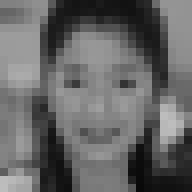
\includegraphics[width=1in]{face1}
\hspace{0.1in}
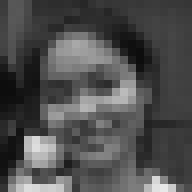
\includegraphics[width=1in]{face2}
\hspace{0.1in}
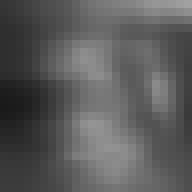
\includegraphics[width=1in]{nonface1}
\hspace{0.1in}
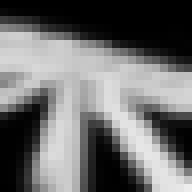
\includegraphics[width=1in]{nonface2}

\end{frame}


\begin{frame}
\frametitle{Introduction}
\framesubtitle{Classification by template matching}

As an example of how we might approach object finding and recognition,
consider \alert{template matching}:
\begin{itemize}
\item We are looking for some kind of object in an image.
\item But we don't know \alert{where} the object is.
\item We might sweep a \alert{detection window} over the image and
  classify each possible window.
\item But we don't know \alert{what orientation} the object is in.
\item For each detection window, we might consider several possible
  orientations.
\item But we don't know \alert{how big} the object is.
\item We might search not only the original image, but successively
  \alert{downscaled} versions of the image.
\end{itemize}

\medskip

This is the \alert{template matching} approach to object recognition.

\end{frame}


\begin{frame}
\frametitle{Introduction}
\framesubtitle{Template matching}

Template matching can get the job done but is plagued with problems:
\begin{itemize}
    \item Speed
    \item Which examples to use as templates
    \item How to evaluate similarity between template and image region?
\end{itemize}

\medskip

In the learning approach, we \alert{let the data decide}.

\end{frame}


\begin{frame}
\frametitle{Introduction}
\frametitle{Necessary ingredients for classification}

In most cases, finding and recognizing objects boils down to
classification.  Classification involves two steps:
\begin{itemize}
\item \alert{Inference}: determining a probability distribution over
  set of hidden variables given a set of observed variables.
\item \alert{Decision making}: determining what to do based on the
  inferred probability distribution.
\end{itemize}

\medskip

\alert{Probabilistic} or \alert{generative} methods make these two
steps explicit.  Example: maximum a posteriori classification of
pixels as skin or not skin.

\medskip

\alert{Black box} methods combine the two steps in an opaque fashion.
Example: support vector machine or neural network classification of
faces.

\medskip

Both types of classifier require some form of \alert{learning}.

\end{frame}


\begin{frame}
\frametitle{Introduction}
\frametitle{Learning}

\begin{block}{Learning}
  Estimating the \alert{parameters} and/or \alert{structure} of a
  probabilistic model from a \alert{training set}.
\end{block}

\medskip

The learning approach is immensely powerful.  Consider the case of
speech recognition (from Bill Freeman):
\begin{itemize}
\item Prior to 1980s, speech recognition techniques were ad hoc.
\item The introduction of statistical models with efficient learning
  algorithms (HMMs) revolutionized the field.
\item Now \alert{the person with the best training set} wins.
\end{itemize}

\medskip

The same transformation began in computer vision starting around 2000
and is complete today.

\end{frame}


\begin{frame}
\frametitle{Introduction}
\framesubtitle{Feature-based vs.\ deep learning methods}

The 2010's have seen big changes machine learning applications in vision.

\medskip

Prior to 2012 or so: \alert{feature based} approaches were the winners
for most problems.

\medskip

Feature-based methods work in two phases:
\begin{itemize}
\item Given an instance, compute a low-dimensional feature vector
  describing the instance.
\item Pass the feature vector to a classifier.
\end{itemize}

\medskip

The classifier might be a SVM, a Gaussian classifier, a shallow neural
network, or a nearest neighbor classifier.

\end{frame}


\begin{frame}
\frametitle{Introduction}
\framesubtitle{Feature-based vs.\ deep learning methods}

Since 2012, \alert{deep learning} models have completely transformed
the field.

\medskip

The general idea is to move as close as possible to \alert{end-to-end}
learning:
\begin{itemize}
\item The input is handed directly to the model without preprocessing.
\item The model outputs the decision, possibly after a complex,
  multi-step calculation.
\end{itemize}

\medskip

Successful applications that seemed insanely futuristic just a few
years ago include self-driving cars and payments using face
recognition.

\end{frame}


\begin{frame}
\frametitle{Introduction}
\framesubtitle{Feature-based vs.\ deep learning methods}

As of the late 2010's, most deep learning models require parallel
computation with GPUs for real time performance.

\medskip

This gives us a simple decision tree:
\begin{itemize}
\item If a simple feature-based model is sufficient for a given task,
  go with it.
\item Otherwise, if you have \alert{sufficient training data} and
  \alert{sufficient compute power at runtime}, deep learning will win
  every time.
\item Otherwise, if you have \alert{insufficient training data} but
  still have \alert{sufficient compute power at runtime}, you may be
  able to \alert{fine-tune} an existing deep learning model.
\item Otherwise, hand-craft the best feature-based model you can. 
\end{itemize}

\end{frame}


\begin{frame}
\frametitle{Introduction}
\framesubtitle{Supervised learning problems in machine vision}

The most important applications of supervised machine learning in
computer vision are probably \alert{detection},
\alert{classification}, and \alert{segmentation}.

\medskip

\alert{Detection is really just classification}:
\begin{itemize}
\item We may classify each subwindow of an image sequentially
  using a sweep window.
\item We may look for ``interesting'' locations first using some kind
  of interest operator.
\item Or, we may classify all possible locations in parallel.
\end{itemize}

\end{frame}


\begin{frame}
\frametitle{Introduction}
\framesubtitle{Supervised learning problems in machine vision}

Similarly, \alert{segmentation is just classification}:
\begin{itemize}
\item We may classify each \alert{pixel} as a member of the same
  segment as its neighbors or a different segment.
\item In \alert{semantic segmentation}, we attach a specific
  \alert{category label} to each pixel of the image.
\end{itemize}
  
\medskip

The key in all of these cases is to be able to classify an image or a
patch of an image or a pixel of an image.

\medskip

We'll thus first look at some different kinds of simple classifiers
then see how they are applied to machine vision problems.

\end{frame}

%--------------------------------------------------------------------
\section{Classifiers for machine vision}
%--------------------------------------------------------------------

\begin{frame}
\frametitle{Classifiers for machine vision}
\framesubtitle{Explicit probability models}

There are two distinct kinds of classifier induction algorithms:

\medskip

\begin{itemize}
\item[-] \alert{Explicit probability models} or \alert{generative
  models} use the training set to build a probability model for the
  likelihood $P(\vec{x} \mid y)$ or the posterior $P(y \mid \vec{x})$.

  \smallskip
  Example: estimate the parameters of a Gaussian distribution from
  each example set.

  \smallskip
  Limitation: if the probability model is not sufficiently powerful to
  capture the true distribution of the members of each class, we might
  not get a good decision boundary.

\end{itemize}

\end{frame}

%--------------------------------------------------------------------
\begin{frame}
\frametitle{Classifiers for machine vision}
\framesubtitle{Direct decision boundary induction}

\begin{itemize}
\item[-] \alert{Direct decision boundary induction} tries to find a
  good decision boundary without the intermediate step of probability
  modeling.

  \smallskip
  Example: support vector machines (SVMs).

  \smallskip
  Limitation: if the induction algorithm is not powerful enough to
  model the decision boundary accurately, we might not get a good
  decision boundary.  If it is \alert{too powerful} it might pay too
  much attention to the training set without generalizing.
\end{itemize}

\end{frame}

%--------------------------------------------------------------------
\begin{frame}
\frametitle{Classifiers for machine vision}
\framesubtitle{Example: normal class-conditional densities}

As an explicit probabilistic model, the \alert{multidimensional
  Gaussian density} is
\[ P(\vec{x}) = \frac{1}{(2 \pi)^{N/2}|\Sigma|^{1/2}} \exp \left(
  -\frac{1}{2} (\vec{x}-\vec{\mu})^T \Sigma^{-1} (\vec{x}-\vec{\mu})
\right) \]

where $\vec{\mu}$ is the mean and $\Sigma$ is the covariance of the
distribution.  For a $N$-class classification problem, we have
distinct means and covariances $\vec{\mu}_k, \Sigma_k, k \in 1\ldots
N$.  Using the training set we estimate the parameters of the Gaussian
class-conditional densities $P(\vec{x} \mid k)$:
\[ \vec{\mu}_k = \frac{1}{N_k} \sum_{i=1}^{N_k} \vec{x}_{ki}
\mbox{\hspace{0.4in}}
   \Sigma_k = \frac{1}{N_k-1} \sum_{i=1}^{N_k} (
   \vec{x}_{ki}-\vec{\mu}_k) (\vec{x}_{ki}-\vec{\mu}_k)^T \]

Now what is the appropriate decision rule?  Hint: if $a<b$, $\log a <
\log b$.

\end{frame}

%--------------------------------------------------------------------
\begin{frame}
\frametitle{Classifiers for machine vision}
\framesubtitle{Example: nearest neighbor}

As an example of a direct decision boundary induction technique,
consider \alert{nearest neighbors}:
\begin{block}{$(k,l)$ nearest neighbors algorithm}
Find the
$k$ nearest neighbors of $\vec{x}$ in the training set, and return the
most common category in the set, if it appears at least $l$ times.
\end{block}

\medskip

Nearest neighbors often performs very well, \alert{without having to
  model} the data's probability distribution.

\end{frame}

%--------------------------------------------------------------------
\begin{frame}
\frametitle{Classifiers for machine vision}
\framesubtitle{Example: nearest neighbor}

Nearest neighbors has one main limitation: computing Euclidean
distance to \alert{every element} of the training set is expensive,
especially if the feature space is high dimensional.

\medskip

Research issues include avoiding calculating distances to every
element of the training set, what distance measures are appropriate,
and how to remove superfluous training set items.

\medskip

One example was Beis and Lowe's ``best bin first'' approximate nearest
neighbors algorithm used to quickly get correspondences for SIFT keypoints.

\end{frame}

%--------------------------------------------------------------------
\begin{frame}
\frametitle{Classifiers for machine vision}
\framesubtitle{Example: classification with histograms}

As another example of an explicit probabilistic method, consider
a Bayesian \alert{skin pixel classifier}:
\begin{itemize}
\item \alert{Training}: Construct a histogram of skin pixels and
  non-skin pixels in HS space.
\item \alert{Classification}: Classify each pixel as skin or non-skin
  based on which model has the highest histogram count.
\end{itemize}

The skin histogram gives an estimate of $P(\vec{x}=(h, s)^T \mid
\mbox{skin})$ and the non-skin histogram gives an estimate of
$P(\vec{x}=(h, s)^T \mid \mbox{not skin})$.

\medskip

Picking the category with the highest histogram count corresponds to
Bayesian classification under \alert{uniform category priors}.

\end{frame}

%--------------------------------------------------------------------
\section{Estimating and improving performance}
%--------------------------------------------------------------------

\begin{frame}
\frametitle{Estimating and improving performance}
\framesubtitle{Use a separate test set}

How well are wee doing in a classification task?

\medskip

\alert{Training set loss/accuracy} is one measure, but if the model
has high VC dimension, it will tend toward \alert{overfitting}.

\medskip

There are many techniques for avoiding overfitting (early stopping,
weight decay, drop-out, etc.).

\medskip

However, to determine if these techniques are working properly, we
need to \alert{measure} the degree to which we are overfitting.

\medskip

The main technique for measuring overfitting is to reserve a
\alert{test set} that is not used during training.

\medskip

The test set should be independent of the training set. It will
indicate how well our system will \alert{generalize} to new unseen
data.

\end{frame}


\begin{frame}
\frametitle{Estimating and improving performance}
\framesubtitle{Use a separate test set}

\myfig{3.5in}{error}{}

\end{frame}


\begin{frame}
\frametitle{Estimating and improving performance}
\framesubtitle{Use separate validation and test sets}

Most models have two kinds of parameters: \alert{learned} or
\alert{tuned} parameters and \alert{hyperparameters} or \alert{free
  parameters}.

\medskip

Learned parameters include weights in a neural network, the elements
of the hyperplane's normal vector in a SVM, and each frequency in a
histogram.

\medskip

Hyperparameters include the number of units/layers in a neural network,
the error tolerance of a SVM, and the number of bins in the histogram.

\medskip

To \alert{measure and control overfitting} of the tuned parameters of
a model, \alert{we need a test set}.

\medskip

To \alert{compare different models with different hyperparameters},
\alert{we need a test set}.

\end{frame}


\begin{frame}
\frametitle{Estimating and improving performance}
\framesubtitle{Use separate validation and test sets}

In practice, then, we need \alert{three data sets}:
\begin{itemize}
\item \alert{Training set}: the data set on which we minimize the cost function,
  by gradient descent or another method.
\item \alert{Validation set}: an independent data set used for estimating
  the generalization accuracy of a trained model, measuring overfitting,
  and performing early stopping.
\item \alert{Test set}: an independent data set used to compare
  different models with different hyperparameters.
\end{itemize}

\medskip

Note, however, that if you use your test set more than once, it
becomes a kind of training/validation set, and you are performing
\alert{data snooping}.

\medskip

To be completely fair, then, it might be wise to reserve a fourth,
\alert{final final test set} representing unseen data that is
\alert{only used once}, when model selection is complete.

\end{frame}


\begin{frame}
\frametitle{Estimating and improving performance}
\framesubtitle{Cross validation}

Reserving a test set wastes valuable training items, so
\alert{cross validation} is useful when data is scarce.

\end{frame}

%--------------------------------------------------------------------
\begin{frame}
\frametitle{Estimating and improving performance}
\framesubtitle{Bootstrapping}

The best way to improve performance is almost always to
\alert{increase the size of the training set}.

\medskip

But collecting \alert{new training data} can be \alert{expensive}, and
training on unneeded data might waste time.

\medskip

\alert{Bootstrapping} selects new items for training according to
\alert{how close} they are to the \alert{existing classifier's}
decision boundary.

\end{frame}

%--------------------------------------------------------------------
\section{Feature selection and feature learning}
%--------------------------------------------------------------------

\begin{frame}
\frametitle{Feature selection and feature learning}
\framesubtitle{Motivation}

In a histogram-based skin classification problem, we might decide to
build our histograms in the H-S plane of the HSV color model.

\medskip

\fbox{For more complex problems, how do we decide what features
  to use for our classifier?}

\begin{enumerate}

  \item \alert{Hand-crafted features}: SIFT descriptors,
    principal components, local receptive field histograms, edge
    filter histograms, 30+ years of research and thousands of choices!
  \item \alert{End-to-end feature learning with deep
    learning}:  Give the data complete control over what the features
    should be.
  \item (A middle ground) \alert{Feature selection from a family of
    features}: Put some intelligent design into a large family of
    possible features, then let the data decide which ones to use.
\end{enumerate}

\medskip

Feature selection is appropriate when runtime resources are
constrained or the labeled data you have access to is insufficient for
end-to-end learning.

\end{frame}


\begin{frame}
\frametitle{Feature selection and feature learning}
\framesubtitle{Feature selection principles}

\begin{block}{Feature selection prinicples}
\begin{itemize}
\item Find features \alert{related to the classification} you want to
  make.
\item Keep the \alert{number} of features as \alert{small} as possible.
\item Do not use \alert{correlated} features.
\end{itemize}
\end{block}

\end{frame}


\begin{frame}
\frametitle{Feature selection and feature learning}
\framesubtitle{Linear feature selection in vision}

The simplest features are \alert{linear combinations} of specific
image pixels.  Linear combinations are good computationally.

\begin{itemize}
\item Or we could do \alert{linear dimensionality reduction} to
  transform a large number of correlated inputs into a smaller feature
  space.
\item We could \alert{learn} linear features that are good for a
  classification task.
\end{itemize}

\medskip

Next we will see how to learn features linear features in the context
of a \alert{face detection} task.

\medskip

This technique of learning fast linear features is due to Viola and
Jones.

\medskip

The combination of fast linear features, ensemble learning, and a decision
cascade enabled the first real-time face detector, on 2000-era hardware.

\medskip

The principles are still valid today.

\end{frame}


\begin{frame}
\frametitle{Feature selection and feature learning}
\framesubtitle{Detection as classification}

We already discussed how \alert{object detection} can be considered a
\alert{classification problem}.

\medskip

We slide a detection window at multiple scales over the image, then
for each window, we extract a set of simple features and classify the
result as a positive or negative.

\end{frame}


\begin{frame}
\frametitle{Feature selection and feature learning}
\framesubtitle{Viola and Jones}

Viola and Jones' famous method for face detection was the first real
time face detection method.

\medskip

Viola, P., and Jones, M.J.\ (2001), ``Robust real-time face detection,''
\textit{International Journal of Computer Vision} 57(2):137--154.

\medskip

The method is based on learning of features for a sliding window
classifier.

\medskip

It builds a strong classifier by combining many simple classifiers
called \alert{decision tree stumps}, which use just a single feature
and are extremely easy to train.

\medskip

By building a powerful classifier out of an ensemble of simple
classifiers using a single feature each, the method performs feature
selection \alert{at the same time} as it is learning the decision
boundary.

\medskip

Before we can understand their method, we need to understand the
underlying learning algorithm, \alert{AdaBoost}.

\end{frame}


\begin{frame}
\frametitle{Feature selection and feature learning}
\framesubtitle{Combining models}

Simple direct decision boundary induction approaches like the linear
SVM do not work for complex problems with \alert{many features} and
\alert{nonlinear decision boundaries}.

\medskip

To address this issue we have two directions to go in:
\begin{itemize}
\item Build a \alert{more complex model} using a more powerful
  classifier such as a neural network or a kernelized support vector
  machine;
\item Stick with a simple classifier, but use \alert{more than one
    classifier} to make up for the deficiencies of a single, simple
  classifier.
\end{itemize}

\medskip

Benefits of multiple simple classifiers:
\begin{itemize}
\item The individual classifiers are \alert{easy} and \alert{quick} to
  train.
\item Simplicity means there is less risk of \alert{overfitting the
    training set} than with a universal classifier.
\item Feature selection is \alert{built in} (for some classifiers).
\end{itemize}

\end{frame}


\begin{frame}
\frametitle{Feature selection and feature learning}
\framesubtitle{Combining classifiers}

There are two basic approaches to combining classifiers.
First we train $L$ different models,
then at classification time, we either
\begin{itemize}
\item run the input pattern $\vec{x}$ through all classifiers and
  somehow \alert{average their predictions}, or
\item use $\vec{x}$ to \alert{select just one} of the $L$ classifiers
  to perform the job.
\end{itemize}

\medskip

We focus on a variant of the first idea, a \alert{committee}.

\end{frame}

\begin{frame}
\frametitle{Feature selection and feature learning}
\framesubtitle{Committees: the idea}

The idea of a committee is to \alert{average the predictions} of a set
of \alert{individual} models.

\medskip

We could, for example, train multiple classifiers, each using a
\alert{different data set}, then put them together.

\medskip

The goal is for the errors of different classifiers to \alert{average
  out}.

\end{frame}

\begin{frame}
\frametitle{Feature selection and feature learning}
\framesubtitle{Bagging}

The trouble with the committee idea is that we only have one data set, and
we would like to train on all of the data.

\medskip

How can we get \alert{different committee members} that are really
different from each other?

\medskip

One way, called \alert{bootstrapping} or \alert{bagging}, is to
randomly sample $N$ items from our $N$-item data set $\vec{X}$ with
replacement.

\medskip

Repeating this $M$ times, we get $M$ different data sets, which we can
then use to train $M$ different classifiers $y_m(\vec{x})$.  Then the
final combined model is
\begin{equation*}
y_{COM}(\vec{x}) = \frac{1}{M} \sum_{m=1}^M y_m(\vec{x})
\end{equation*}

\end{frame}

\begin{frame}
\frametitle{Feature selection and feature learning}
\framesubtitle{Boosting}

It can be shown that in bagging, if the \alert{errors made by the
  different models are uncorrelated} and the average expected error of
the individual classifiers is $E_{AV}$, then the expected error of the
combined model is $\frac{1}{M}E_{AV}$.

\medskip

The gain is huge, but in practice the assumption of uncorrelated
errors \alert{does not hold}.

\medskip

\alert{Boosting} methods are a more sophisticated means to introducing
variance among committee members.

\end{frame}


\begin{frame}
\frametitle{Feature selection and feature learning}
\framesubtitle{Boosting: the idea}

Boosting combines multiple \alert{base} classifiers to produce a
committee whose performance is possibly better than any of the
individual committee members.

\medskip

The most widely used boosting method is Freund and Schapire's (1996)
\alert{AdaBoost} (adaptive boosting) algorithm.

\medskip

Boosting combines multiple \alert{weak learners} whose performance need
only be \alert{slightly better than random}.

\medskip

The main difference between boosting and bagging is that the learners
are trained \alert{sequentially}, where each classifier is trained on
a \alert{weighted} form of the training set, and the weights
\alert{depend on the performance of the previous classifiers}.

\end{frame}


\begin{frame}
\frametitle{Feature selection and feature learning}
\framesubtitle{Boosting}

\myfig{3.25in}{Bishop-fig14-1.pdf}{Bishop (2006), Fig.\ 14.1}

\end{frame}


\begin{frame}
\frametitle{Feature selection and feature learning}
\framesubtitle{Boosting}

The scheme:
\begin{itemize}
\item We have a two-class classification problem with \alert{training
    data} $\vec{x}_1,\ldots,\vec{x}_N$ and corresponding binary
  \alert{targets} $t_1,\ldots,t_N$ where $t_n \in \{-1,1\}$.
\item We additionally give each data point $\vec{x}_n$ a
  \alert{weighting parameter} $w_n$ which is initialized to $1/N$ for
  all points.
\item Suppose we have a \alert{training procedure} that produces a
  base classifier $y(\vec{x}) \in \{-1,1\}$ using the weighted data.
\item At each stage, AdaBoost trains a new classifier using weights
  that are adjusted to give \alert{more weight} to points
  \alert{misclassified} by the previous classifier.
\item Finally the base classifiers are combined into a committee with
  \alert{weighted majority voting}.
\end{itemize}

\end{frame}


\begin{frame}
\frametitle{Feature selection and feature learning}
\framesubtitle{Boosting}

\begin{block}{AdaBoost: Objective}
Given a training data set $\vec{x}_1,\ldots,\vec{x}_N$, corresponding
binary targets $t_1,\ldots,t_N$ where $t_n \in \{-1,1\}$, and a method
for constructing a weak classifier minimizing the weighted
classification error, construct a strong classifier $Y_M(\vec{x})$.
\end{block}

\end{frame}


\begin{frame}
\frametitle{Feature selection and feature learning}
\framesubtitle{Boosting}

\begin{block}{AdaBoost: Algorithm (Bishop, 2006, p.\ 658)}
\begin{itemize}
\item[(i)] Initialize weights $\{w_n\}$ by setting $w_n^{(1)} = 1/N$
  for $n=1,\ldots,N$.
\item[(ii)] For $m=1,\ldots,M$:
  \begin{itemize}
  \item[(a)] Fit a classifier $y_m(\vec{x})$ to the training data by
    minimizing the weighted error function
    \begin{equation*}
    J_m=\sum_{n=1}^N w_n^{(m)}I(y_m(\vec{x}_n)\not= t_n).
    \end{equation*}
    Here $I(\cdot)$ is the indicator function, equal to 1 when its
    argument is true and equal to 0 otherwise.
  \end{itemize}
\end{itemize}
\end{block}

\end{frame}


\begin{frame}
\frametitle{Feature selection and feature learning}
\framesubtitle{Boosting}

\begin{block}{AdaBoost: Algorithm (Bishop, 2006, p.\ 658, continued)}
\begin{itemize}
\item[(ii)] continued:
  \begin{itemize}
  \item[(b)] Evaluate the quantities
    \begin{equation*}
    \epsilon_m=\frac{\sum_{n=1}^N w_n^{(m)}I(y_m(\vec{x}_n)\not=t_n)}
                    {\sum_{n=1}^N w_n^{(m)}}
    \end{equation*}
    then use them to evalulate
    \begin{equation*}
    \alpha_m = \ln\left\{\frac{1-\epsilon_m}{\epsilon_m}\right\}.
    \end{equation*}
  \item[(c)] Update the weights
    \begin{equation*}
    w_n^{(m+1)} = w_n^{(m)}\exp\{\alpha_m I(y_m(\vec{x}_n)\not=t_n)\}
    \end{equation*}
  \end{itemize}
\end{itemize}
\end{block}

\end{frame}


\begin{frame}
\frametitle{Feature selection and feature learning}
\framesubtitle{Boosting}

\begin{block}{AdaBoost: Algorithm (Bishop, 2006, p.\ 658, continued)}
\begin{itemize}
\item[(iii)] Make predictions using the final model
  \begin{equation*}
  Y_M(\vec{x}) = \sign \left( \sum_{m=1}^M \alpha_m y_m(\vec{x})
  \right).
  \end{equation*}
\end{itemize}
\end{block}

\end{frame}


\begin{frame}
\frametitle{Feature selection and feature learning}
\framesubtitle{Intuitive view of the algorithm}

Some intuitive observations about the algorithm:
\begin{itemize}
\item The first classifier $y_1(\vec{x})$ is trained with uniform
  weights, so it will be a typical classifier trained on $\vec{X}$.
\item In step (ii)(c), we see that $w_n^{(m)}$ is \alert{held
    constant} for cases where $y_m(\vec{x}_n) = t_n$ and
  \alert{increased} for cases where $y_m(\vec{x}_n) \not= t_n$.
\item This forces \alert{later classifiers} to put \alert{more
    emphasis} on training examples that have been
  \alert{misclassified} by previous classifiers.
\item $\epsilon_m$ represents the weighted error measure for
  classifier $m$.
\item In step (ii)(c), $\epsilon_m$ is used to give \alert{even more
    weight} to misclassified examples when $y_m(\vec{x})$ is good.
\item In step (iii), $\epsilon_m$ is used to give a \alert{bigger
    vote} to classifiers that had \alert{low error} during training.
\end{itemize}

\end{frame}


\begin{frame}
\frametitle{Feature selection and feature learning}
\framesubtitle{Example}

Here is an example with \alert{decision stump} learners.  Color
represents class and radius represents weight. The dashed boundary is
the decision surface for the $m$th classifier, and the green boundary
is the decision surface for the combined classifier.

\medskip

\begin{columns}
\column{1.5in}
\myfig{1.6in}{Bishop-fig14-2a.pdf}{}
\column{1.5in}
\myfig{1.6in}{Bishop-fig14-2b.pdf}{Bishop (2006), Fig.\ 14.2(a)-(c)}
\column{1.5in}
\myfig{1.6in}{Bishop-fig14-2c.pdf}{}
\end{columns}

\end{frame}


\begin{frame}
\frametitle{Feature selection and feature learning}
\framesubtitle{Example}

\begin{columns}
\column{1.5in}
\myfig{1.6in}{Bishop-fig14-2d.pdf}{}
\column{1.5in}
\myfig{1.6in}{Bishop-fig14-2e.pdf}{Bishop (2006), Fig.\ 14.2(d)-(f)}
\column{1.5in}
\myfig{1.6in}{Bishop-fig14-2f.pdf}{}
\end{columns}

\end{frame}


\begin{frame}
\frametitle{Feature selection and feature learning}
\framesubtitle{Formal view of the algorithm}

Friedman et al. (2000) found a straightforward explanation of
AdaBoost.

\medskip

Suppose we have an error function
\begin{equation*}
E = \sum_{n=1}^N \exp \{ -t_n f_m(\vec{x}_n) \}
\end{equation*}
where $f_m(\vec{x})$ is the linear combination of base classifiers
\begin{equation*}
f_m(\vec{x}) = \frac{1}{2} \sum_{l=1}^m \alpha_l y_l(\vec{x})
\end{equation*}
and $t_n \in \{-1,1\}$ are the targets.  What if we minimize $E$ with
respect to weighting coefficients $\alpha_l$ and parameters of
$y_l(\vec{x})$?

\end{frame}


\begin{frame}
\frametitle{Feature selection and feature learning}
\framesubtitle{Formal view of the algorithm}

It turns out that if we fix the base classifiers
$y_1(\vec{x}),\ldots,y_{m-1}(\vec{x})$, we find that $y_m(\vec{x})$,
$\alpha_m$, and $w_n^{(m+1)}$ as defined by AdaBoost exactly minimize
$E$ (see Bishop, 2006, pages 659--661).

\medskip

This \alert{exponential error function} is different from the
\alert{cross-entropy} error function typically used in machine learning:
\begin{equation*}
E = -\sum_{n=1}^N \{ t_n \ln y(\vec{x}_n) + (1-t_n)\ln (1-y(\vec{x}_n)) \}
\end{equation*}
with targets $t_n \in \{0,1\}$.

\end{frame}


\begin{frame}
\frametitle{Feature selection and feature learning}
\framesubtitle{Formal view of the algorithm}

Exponential error is mainly interesting because it happens to lead to
AdaBoost!

\medskip

It has a few disadvantages compared to cross entropy:
\begin{itemize}
\item Exponential error puts \alert{more weight} on misclassified data
  points, making it \alert{more sensitive} to outliers or mislabeled
  inputs.
\item Exponential error \alert{cannot} be interpreted as a \alert{log
    likelihood} function of any simple probabilistic model (we prefer
  maximum likelihood estimation over ad-hoc methods).
\item Exponential error does not generalize to \alert{multiclass}
  problems.
\end{itemize}

\medskip

However, by replacing the error function, we can derive a variety of
boosting algorithms with desired properties.

\medskip

There has been a lot of research on how to get the good generalization
of AdaBoost on multiclass problems and in situations with outliers.

\end{frame}


\begin{frame}
\frametitle{Feature selection and feature learning}
\framesubtitle{How can we use AdaBoost for face detection?}

The Viola and Jones face detection algorithm works like this:
\begin{itemize}
\item Sweep a small \alert{detection window} over the image at multiple
  scales.
\item For each candidate face location,
  \begin{itemize}
  \item Extract a set of \alert{features}
    of the pixel values in the detection window.  A feature is just an
    arbitrary (usually but not always linear)
    mathematical function of the pixels in the detection window.
  \item Based on the set of feature values, \alert{decide}
    whether the image patch
    contains a face or not.
  \end{itemize}
\item Group together nearby detections and eliminate overlapping detections.
\end{itemize}

\end{frame}


\begin{frame}
\frametitle{Feature selection and feature learning}
\framesubtitle{How does it work?}

The genius of the method is three main ideas:
\begin{itemize}
\item They came up with a \alert{type
  of feature} that can be computed extremely fast and is effective in
  the decision step.
\item They used an existing method for \alert{learning} which features from
  an enormous set of possible features are effective and how to combine
  them.
\item They came up with a way to quickly \alert{discard}
  detection window locations
  unlikely to contain faces.
\end{itemize}

\medskip

Before Viola and Jones: effective but agonizingly slow face detection.

\medskip

After Viola and Jones: face detection is common in commercial products
such as digital cameras.

\end{frame}


\begin{frame}
\frametitle{Feature selection and feature learning}
\framesubtitle{Features}

The \alert{features}
are simple binary convolution filters combined with a threshold:

\medskip

\centerline{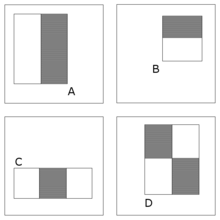
\includegraphics[width=2in]{features}}

\medskip

These are called Haar-like filters and can be computed extremely quickly
using an \alert{integral image}.

\end{frame}


\begin{frame}
\frametitle{Feature selection and feature learning}
\framesubtitle{Rapidly discarding detection windows}

The method for discarding detection windows is to arrange the
AdaBoost classifiers into a \alert{cascade}:

\medskip

\centerline{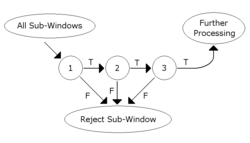
\includegraphics[width=2in]{cascade}}

\medskip

Windows unlikely to be faces are quickly rejected, and windows more likely to
be faces are given more consideration.

\end{frame}


\begin{frame}
\frametitle{Feature selection and feature learning}
\framesubtitle{Summary}

To put the pieces together, we have a \alert{learning} phase and a
\alert{runtime} phase.

\medskip

In the learning phase, we collect thousands of images of faces and non faces
and run AdaBoost with exhaustive search over the set of possible
Haar-like features.

\medskip

This part took days on a compute cluster in the 2000s. Nowadays, training
time is small compared to large CNN models.

\medskip

In the runtime phase, we simply capture images, sweep the detection window
over the image, and apply the feature cascade to determine if the window
contains a face or not.

\medskip

In a final cleanup phase we group nearby detections and eliminate overlapping
detections.

\medskip

Try the ``haarcascade'' sample in the OpenCV distribution.

\end{frame}

%--------------------------------------------------------------------
\section{HOG}
%--------------------------------------------------------------------

\begin{frame}{HOG}{Introduction}

  In 2005, Dalal and Triggs introduced another object detector that we
  still use today.

  \medskip

  Basic idea:
  \begin{itemize}
  \item Apply the multiscale scan window technique
  \item For each window, extract a SIFT-like descriptor for a rectangular
    subregion of the image
  \item Classify the resulting descriptor as object or not object using a linear SVM
  \end{itemize}

  More detailed pipeline:

  \medskip
  
  \myfig{4.5in}{dalal-fig1}{Dalal and Triggs (2005), Fig.\ 1}
  
\end{frame}


\begin{frame}{HOG}{Training data}

  Training sets sizes for HOG detectors usually range in the 1000s.

  \medskip

  Dalal and Triggs used a dataset of 1239 positive patches and 1218
  images without people.

  \medskip

  Initial negative set was 12,180 random patches from the negative images.

  \medskip

  False positives from exhaustive search with intial detector were
  added to the negative set for final training.

  \medskip
  
  Sample positives for human detection:

  \medskip

  \myfig{4.5in}{dalal-fig2}{Dalal and Triggs (2005), Fig.\ 2}

\end{frame}


\begin{frame}{HOG}{Evaluation criteria}

  We have already discussed how important it is to have a very high
  classification accuracy when performing object detection.

  \medskip
  
  How to evaluate a detector? There are two criteria:
  \begin{itemize}
  \item Hit rate
  \item False positive rate
  \end{itemize}

  \medskip

  There are many methods to combine hit rate and FP rate into one number.
  
  \medskip

  Dalal and Triggs use the \alert{miss rate at $10^{-4}$ false
    positives per window} as the criterion.
  
\end{frame}


\begin{frame}{HOG}{Details: color normalization}

  Dalal and Triggs found that detectors work better with color information.

  \medskip

  Same process is applied separately to the R, G, and B channels.

  \medskip

  Gamma correction is used to increase contrast in darker regions of the
  image and reduce contrast in brighter regions.

  \medskip

  Square root correction
  performed better than log correction.

\end{frame}


\begin{frame}{HOG}{Details: gradient calculation}

  Many methods to calculate the gradient were tried.

  \medskip

  1-D gradient filters, i.e., $\begin{bmatrix} -1 & 0 & 1 \end{bmatrix}$,
  without any image smoothing worked best.

  \medskip

  The gradient is performed over the whole image before the scan
  window is applied.

  \medskip

  Color images are collapsed to a single plane by taking, for each
  pixel, the gradient with the largest norm over the three color
  channels. [Clever!]
  
\end{frame}


\begin{frame}{HOG}{Details: orientation binning}

  Each pixel's gradient \alert{votes} for a particular gradient orientation.

  \medskip

  Gradients are binned (a histogram is calculated) over small \alert{cells}.

  \medskip

  The best voting strategy was to have the vote proportional to the
  magnitude of the gradient.

  \begin{columns}

    \column{3in}

  Votes are split with bilinear interpolation over neighboring bins to
  avoid aliasing.

  \medskip

  More orientation bins (up to 9) seems to help.

  \alert{Unsigned orientations} ($0^\circ$ to $180^\circ$) work best
  for human detection, whereas \alert{signed orientations} ($0^\circ$
  to $360^\circ$) work best for some other classes (cars and motorbikes).

  \column{1.5in}

    \myfig{1in}{dalal-hist}{}

  \end{columns}
  
\end{frame}


\begin{frame}{HOG}{Details: block contrast normalization}

  Images have different levels of contrast in different regions.

  \medskip

  For object classification, usually, the \alert{relative} magnitude
  of the gradients is what's important, not the absolute magnitudes.

  \medskip

  \alert{Local contrast normalization} helps us get accurate texture
  information in both high and low contrast areas.

  \medskip

  Cells are grouped into \alert{blocks} (6$\times$6 cells grouped into
  3$\times$3 blocks seems to work well), over which the gradient
  orientation histograms are summed up and normalized.

  \medskip

  Normalization turns out to be critical for good performance. Among
  many methods, L2 normalization ($\vec{v} \leftarrow \vec{v} /
  \sqrt{\|\vec{v}\|^2_2 + \epsilon^2}$) is found to work as well or better
  than other methods.

\end{frame}


\begin{frame}{HOG}{Details: image patch and classifier}

  Dalal and Triggs find that a 64$\times$128 detection window with 16 pixels of border around the person in the patch works best.

  \medskip

  The SVM is a soft margin linear hyperplane classifier with $c = 0.01$.

  \medskip

  The Gaussian RBF kernel gives better performance (3\% improvement in
  the miss rate at $10^{-4}$ FPPW) but requires a much higher runtime
  [recall why RBF increases runtime so much?].
  
\end{frame}


\begin{frame}{HOG}{Results}

  \myfig{4.5in}{dalal-fig6}{Dalal and Triggs (2005), Fig.\ 6}

  \medskip

  Visualization of the HOG descriptor is useful. (a) Average gradient
  over training examples. (b) Maximum positive SVM weight in each
  block of the descriptor. (c) Maximum negative weight in each
  block. (d) Sample test image. (e) HOG descriptor of image in
  (d). (f,g) The HOG descriptor weighted by positive and negataive SVM
  weights.
  
\end{frame}


\begin{frame}{HOG}{Summary}

  The HOG paper is a beautiful example of how to carefully engineer a
  machine vision system. Everyone should read it!

  \medskip

  HOG detectors have competitive performance even today.

  \medskip

  See the HOG implementation in OpenCV, and try the ``peopledetect''
  sample.

\end{frame}


\begin{frame}{HOG}{What's next?}

  HOG represents a pinnacle in the development of
  feature-based methods for object detection. HOG sadly
  may have been \alert{the last great feature-based method} in machine
  vision!

  \medskip

  Remember that in machine learning, rather than hand-crafting
  classification rules, we \alert{let the data decide} what the
  parameters should be.

  \medskip
  
  To further improve classifier performance in difficult, cluttered
  environments, we need to return to Viola and Jones' idea of letting
  the data decide not only the parameters of the final classifier, but
  also to decide \alert{what features are best for a particular task}.

  \medskip

  This, of course, leads us to neural networks and \alert{end-to-end}
  learning.

\end{frame}


%--------------------------------------------------------------------
\section{Convolutions}
%--------------------------------------------------------------------

\begin{frame}{Convolutions}{Continuous convolution}

  \textit{Note: this material on CNNs is repeated from Recent
	Trends in Machine Learning, for reference.}

  \medskip

  \alert{Convolutional neural networks} (CNNs) are good for data with
  a known grid-like topology:
\begin{itemize}
\item Time series form 1-D grids.
\item Images form 2-D grids.
\end{itemize}

Mathematically: convolution is an operation on \alert{two functions}
with a \alert{real-valued} (possibly vector-valued) argument.

\end{frame}


\begin{frame}{Convolutions}{Continuous convolution}

\begin{block}{Continuous convolution for smoothing (Goodfellow et al., 2016)}
We might use convolution for smoothing a 1-D function such as
continuous noisy measurements $x(t)$ of the linear position of a
spaceship:

$$ s(t) = \int x(a) w(t-a) da $$

$$ s(t) = (x * w)(t) $$

\end{block}

$w(\cdot)$ in the smoothing example:
\begin{itemize}
  \item Should be a
\alert{probability density function} to make it a \alert{weighted average}.
\item Should be \alert{0} for negative arguments (the future)
\end{itemize}

\medskip

There are many other applications of continuous convolution.

\end{frame}


\begin{frame}{Convolutions}{Discrete convolution}

  Now we move to \alert{discrete} convolution.

  $x(t)$ is assumed to be a discrete sample from some underlying
  continuous function taken at regular spatial or temporal intervals.

  \medskip
  
  We'll call $x(t)$ the \alert{input} and $w(t)$ the \alert{kernel}.

  \medskip

  The output is usually called a \alert{feature map}.

  \medskip
  
  The continuous integral becomes a \alert{discrete sum}:

  $$ s(t) = (x * w)(t) = \sum_{a = -\infty}^{\infty} x(a) w(t-a) $$

\end{frame}


\begin{frame}{Convolutions}{Multidimensional convolutions}

In a ML application, the input is an arbitrary \alert{multidimensional
  array of data} and the kernel is a \alert{multidimensional array of
  parameters} adapted by the learning algorithm.

\medskip

Multidimensional arrays are called \alert{tensors}.

\medskip

The theoretically infinite functions are assumed 0 everywhere but in
the finite set of points we have stored.

\medskip

Example: a two-dimensional image $I(\cdot,\cdot)$ would best be processed by a
two-dimensional kernel $K(\cdot,\cdot)$:

$$ S(i,j) = (I * K)(i, j) = \sum_m \sum_n I(m,n)K(i-m,j-n). $$

\end{frame}


\begin{frame}{Convolutions}{Multidimensional convolutions}

Convolution is \alert{commutative}, so we can equivalently write

$$ S(i,j) = (I * K)(i,j) = (K * I)(i,j) =
\sum_m \sum_n I(i-m,j-n)K(m,n).$$

This version is easier to implement, as the loop is over the smaller
number of non-zero values in $K(\cdot,\cdot)$.

\end{frame}


\begin{frame}{Convolutions}{Cross-correlation vs.\ convolution}

Note that in both $I * K$ and $K * I$, as the index into the
input \alert{increases}, the input into the kernel \alert{decreases},
and vice versa.

\medskip

We have \alert{flipped} the kernel.

\medskip

Flipping the kernel is necessary mathematically for commutativity, but
is not necessary for the actual information processing. Therefore, we
may use \alert{cross-correlation}

$$S(i,j) = (K \star I)(i,j) = \sum_m \sum_n I(i+m,j+n)K(m,n),$$

in which we don't flip the kernel. You will often see cross-correlation
called convolution in machine learning libraries.

\medskip

In this class, when we say ``convolution'' we will normally mean cross
correlation!

\end{frame}


\begin{frame}{Convolutions}{Example}

  2D convolution operations give us the linear response of a 2D filter
  applied to the pixels in a local region of an image.

  \medskip

  See any of many examples on YouTube, such as
  \url{https://www.youtube.com/watch?v=_iZ3Q7VXiGI} !

  \medskip

  The simplest example is edge detection using, for example, Sobel
  filters:

  $$\begin{bmatrix} 1 & 0 & -1 \\ 2 & 0 & -2 \\ 1 & 0 & -1 \end{bmatrix}
  \;\;\;\;\;
  \begin{bmatrix} 1 & 2 & 1 \\ 0 & 0 & 0 \\ -1 & -2 & -1 \end{bmatrix}$$

\end{frame}


\begin{frame}{Convolutions}{Hierarchical feature maps}

  A convolution may apply to the \alert{input} or \alert{a feature map
    from a previous layer}.

  \medskip

  Typically, convolutions apply to all of the feature maps in the
  previous layer: this is called \alert{convolution over volume}.
  \begin{itemize}
  \item For the input: three maps (R, G, and B) or one map (grayscale).
  \item For an inner layer: the number of kernels. This would be,
    e.g., 96 for AlexNet's second convolutional layer, except that
    AlexNet splits into two separate hierarchies so it is 48 for each
    stream.
  \end{itemize}

\end{frame}


\begin{frame}{Convolutions}{Valid region of the convolution}

Example below. Note that we only use the \alert{valid} parts of the
convolution where the kernel fully overlaps the valid part of the
input.

\myfig{2.2in}{goodfellow-fig9-1}{Goodfellow et al. (2016), Figure 9.1}

\end{frame}


\begin{frame}{Convolutions}{Important ideas behind CNNs}

There are three main important ideas behind the success of
convolutional neural networks:
\begin{itemize}
\item Sparse interactions
\item Parameter sharing
\item Equivariant representations
\end{itemize}

(Aside: a benefit of convolutions is that they can be applied to an
input of variable size.)

\end{frame}


\begin{frame}{Convolutions}{Sparse interactions}

  \alert{Sparse interactions}:
  \begin{itemize}
    \item A fully connected layer has \alert{dense}
interactions (every unit interacts with every unit in the previous
layer)
\item A convolutional layer has \alert{sparse} interactions (each
unit in the output feature map interacts only with a few elements of
the input, via the small kernel.
  \end{itemize}

  \medskip
  
  Fewer parameters means \alert{lower memory requirements} and
  \alert{higher statistical efficiency}.

  \medskip
  
  The specific organization of a convolution also means it can be
  implemented efficiently.

  \medskip

  Dense connections from $m$ inputs to $n$ outputs requires $O(mn)$
  time.  With a kernel of size $k$, we only need $O(kn)$ time.

\end{frame}


\begin{frame}{Convolutions}{Sparse interactions}

Sparse interaction example. Unit $x_3$ only affects units
$s_2$, $s_3$, and $s_4$ in the output feature map.
Compare to dense interaction below.

\myfig{2in}{goodfellow-fig9-2}{Goodfellow et al. (2016), Figure 9.2}

\end{frame}


\begin{frame}{Convolutions}{Sparse interactions}

Looking from above,
unit $s_3$ in the output feature map
has a \alert{receptive field} including $x_2$, $x_3$, and $x_4$.

\myfig{2in}{goodfellow-fig9-3}{Goodfellow et al. (2016), Figure 9.3}

\end{frame}


\begin{frame}{Convolutions}{Sparse interactions}


When convolutional layers are formed into hierarchies, a unit in a
deep layer ($g_3$) can be \alert{indirectly connected} to all or most
of the input.

\medskip

\myfig{2.5in}{goodfellow-fig9-4}{Goodfellow et al. (2016), Figure 9.4}

\end{frame}


\begin{frame}{Convolutions}{Parameter sharing}

  \alert{Parameter sharing}:
  \begin{itemize}
    \item Sharing means using the same parameter for more than one interaction
      in a model.
    \item Shared parameters are also often called \alert{tied weights}.
      \item In a convolution, each weight in the kernel
        is \alert{reused} at every position in the input.
  \end{itemize}

  Parameter sharing \alert{increases statistical efficiency}.
  
\end{frame}


\begin{frame}{Convolutions}{Parameter sharing}

With parameter sharing (top), one parameter is used many times.
Without parameter sharing, one parameter is used only once.
\myfig{2.6in}{goodfellow-fig9-5}{Goodfellow et al. (2016), Figure 9.5}

\end{frame}


\begin{frame}{Convolutions}{Parameter sharing}

The representational power of convolution with shared parameters is
clear with the following example of vertical edge detection using a
2-element kernel (-1,1):

\myfig{3in}{goodfellow-fig9-6}{Goodfellow et al. (2016), Figure 9.6}

\end{frame}


\begin{frame}{Convolutions}{Equivariance}

  \alert{Equivariance}:
  \begin{itemize}
  \item A function $f(x)$ is \alert{equivariant} to function $g$ if $f(g(x)) =
    g(f(x))$.
  \item Convolution is equivariant to \alert{translation}.
  \item If $f$ is a convolution operation and $g$ is a translation
    operation, we can see that the convolution of a translated version
    of input $x$ is the same as the translation of the convolution of
    $f$ and the input $x$.
  \end{itemize}

  \medskip
  
  How is equivariance useful?

  \medskip

  For time series: we get the same response to the same event,
  \alert{regardless of when} the event occurs.

  \medskip
  
  For images: we get the same response to a local pattern,
  \alert{regardless of where} in the image it occurs.

  \medskip
  
  Note that convolution is NOT equivariant to scale, rotation, etc.

\end{frame}


\begin{frame}{Convolutions}{Activation / rectification}

  One of the insights of the CNN is to perform convolutions
  \alert{hierarchically}.

  \medskip

  However, a hierarchy of purely \alert{linear} transformations would
  ultimately be equivalent to a single linear transformation, which would
  not give powerful pattern matching capabilities.
  
  \medskip
  
  Generally, then, the result of one convolution in the hierarchy
  should be transformed by a nonlinearity.

  \medskip

  ReLU is the most popular
  nonlinear activation function.

  \medskip

  Hyperbolic tangent and the logistic sigmoid are also possible but
  lead to slower learning, according to Krizhevsky et al.\ (AlexNet).

  \medskip
  
  The resulting feature map may possibly be downscaled by a
  \alert{pooling} operation before it is convolved with higher-level
  filters.
  
\end{frame}


\begin{frame}{Convolutions}{Pooling}

The structure of a CNN usually contains several ``macro'' layers
consisting of a convolution, a nonlinearity especially ReLU, then
pooling. Sometimes a ``layer'' means all three operations, and sometimes
each operation is treated separately.

\myfig{2in}{goodfellow-fig9-7}{Goodfellow et al. (2016), Figure 9.7}

\end{frame}


\begin{frame}{Convolutions}{Pooling}

Pooling makes the output feature map approximately \alert{invariant}
to small translations of the input.

\myfig{1.8in}{goodfellow-fig9-8}{Goodfellow et al. (2016), Figure 9.8}

This is good when we want to know \alert{whether} a feature is in the
input, without knowing precisely \alert{where} it is.

\end{frame}


\begin{frame}{Convolutions}{Pooling}

Pooling \alert{over features} enables invariance to more complex
transformations of the input, such as rotation:
\myfig{3in}{goodfellow-fig9-9}{Goodfellow et al. (2016), Figure 9.9}

\end{frame}


\begin{frame}{Convolutions}{Pooling}

Usually, pooling is combined with downsampling, which reduces the
computational and statistical burden on the next layer.

\medskip

\myfig{3in}{goodfellow-fig9-10}{Goodfellow et al. (2016), Figure 9.10}

\end{frame}


\begin{frame}{Convolutions}{Putting it together}

  \begin{columns}

    \column{2in}

    Some sample CNN architectures, as examples.  Note that practical
networks are deeper, more variable, and have branches.

\medskip

Generally, the kinds of processing we want to do on spatial and temporal
data fit the convolve + pool processing approach, but it may not always
be so. Convolution and pooling may cause \alert{underfitting}.

\column{2.5in}

\myfig{2in}{goodfellow-fig9-11}{Goodfellow et al. (2016), Figure 9.11}

  \end{columns}
  
\end{frame}


\begin{frame}{Convolutions}{Refinements: tensors}

In general, the input, kernel, and output are all tensors of arbitrary
number of dimensions.

\medskip

Images: 2D data with 3 channels (red, green, blue), which may be combined
into mini-batches, giving a 4D tensor as the input.

\medskip

The kernel applied to these data might be a 4D tensor $\mat{K}_{i,j,k,l}$ giving
strength of connection between input channel $i$, output channel $j$, and
offset $(k,l)$ between the output and input unit.  Note that every feature
map $j$ connects with \alert{every} channel $i$ in the input.

\medskip

The output would then be a 3D tensor $\mat{Z}_{i,j,k}$, where $i$ represents
the output channel or feature map and $(j,k)$ indicates the spatial location.

\end{frame}


\begin{frame}{Convolutions}{Refinements: downsampling via stride}

We may also \alert{downsample} during the convolution operation, using
a stride not equal to 1. Example stride of 2:

\myfig{1.8in}{goodfellow-fig9-12}{Goodfellow et al. (2016), Figure 9.12}

\end{frame}


\begin{frame}{Convolutions}{Stride}

  Stride is important:
  \begin{itemize}
  \item Typically, the convolution operation is applied at every pixel
    of the input (stride $=$ 1).
  \item When spatial resolution is less important or neighboring
    receptive fields overlap significantly, we may skip some pixels of
    the input (stride $>$ 1).
  \item Most architectures use a stride of 1 for 3$\times$3
    convolutions and a stride of 1--3 for 5$\times$5 convolution.
  \item The trend: smaller kernels and more layers $\rightarrow$ small
    strides (11$\times$11 convolutions as in AlexNet are not often
    seen).
  \end{itemize}
    
\end{frame}


\begin{frame}{Convolutions}{Refinements: padding}

  \begin{columns}

    \column{1.5in}
    
    We may also \alert{pad} the image so that the valid convolution at
    each layer has the same size as the input to the layer:

    \medskip
    
    Usually, the padding is 0.

    \column{3in}
    
    \myfig{2.5in}{goodfellow-fig9-13}{Goodfellow et al. (2016), Figure 9.13}

  \end{columns}

\end{frame}


\begin{frame}{Convolutions}{Padding}

  Padding is important:
  \begin{itemize}
  \item Without padding, the border would shrink after each
    convolution, and information at the image border would be lost.
  \item In most cases, we should add padding necessary so that the
    output feature map has the same size as the input feature map when
    the stride is 1.
  \item The most common choice for padding seems to be 0-padding.
  \item Matt likes copy-border padding, but most libraries do not implement it.
  \item Most libraries do implement ``reflect'' padding which seems to
    work well (and is better than zero-padding).
  \end{itemize}
  
\end{frame}


\begin{frame}{Convolutions}{Refinements: local connection}

In \alert{unshared convolution}, we perform the same dot product of a
set of weights over a local region in the input, but do not use a shared
kernel.

\medskip

This makes sense when we need local sparse computation but have
no reason to apply the same operation throughout the input.

\end{frame}


\begin{frame}{Convolutions}{Refinements: local connection}

Comparison of local connections, convolution, and full connection:

\myfig{1.8in}{goodfellow-fig9-14}{Goodfellow et al. (2016), Figure 9.14}

\end{frame}


\begin{frame}{Convolutions}{Refinements: organizing by channel}

We may also want separate kernels for each input channel:

\myfig{1.6in}{goodfellow-fig9-15}{Goodfellow et al. (2016), Figure 9.15}

\end{frame}


\begin{frame}{Convolutions}{Refinements: tiled convolution}

Another variation is \alert{tiled convolution} in which we combine
the idea of having separate weights for neighboring positions in the
feature map but also sharing parameters:

\myfig{1.6in}{goodfellow-fig9-16}{Goodfellow et al. (2016), Figure 9.16}

\end{frame}


\begin{frame}{Convolutions}{Refinements: transpose convolution}

\alert{Transpose convolution} means multiplication by the transpose of the
matrix defined by convolution. It is used for
\begin{itemize}
\item Backpropagating error derivatives through a convolutional layer
\item Reconstructing input units from hidden units in an autoencoder
\end{itemize}

\end{frame}


\begin{frame}{Convolutions}{Backpropagation}

Suppose we have a convolution tensor $\mat{K}$ applied to multichannel
tensor $\mat{V}$ with stride $s$: $c(\mat{K},\mat{V},s)$.

\medskip

Suppose the loss function is $\mat{J}(\mat{V},\mat{K})$.

\medskip

Forward propagation gives us $\mat{Z} = c(\mat{K},\mat{V},s)$.

\medskip

$\mat{Z}$ is propagated forward, then during backpropagation, we
receive tensor $\mat{G}$ where
$$\mat{G}_{i,j,k} = \frac{\partial}{\partial \mat{Z}_{i,j,k}}
\mat{J}(\mat{V},\mat{K}) .$$

The derivative of $\mat{J}$ with respect to weight $i,j,k,l$ in $\mat{K}$
is
$$ g(\mat{G},\mat{V},s)_{i,j,k,l} = \frac{\partial}{\partial \mat{K}_{i,j,k,l}}
J(\mat{V},\mat{K}) =
\sum_{m,n} \mat{G}_{i,m,n} \mat{V}_{j,(m-1)\times s+k,(n-1)\times s + l}.$$

\end{frame}


\begin{frame}{Convolutions}{Backpropagation}

The deltas to be backpropgated to previous layers are
$$h(\mat{K},\mat{G},s)_{i,j,k} = \frac{\partial}{\partial \mat{V}_{i,j,k}}
J(\mat{V},\mat{K})$$
$$= \sum_{\substack{l,m\\ \textrm{s.t.} (l-1)\times s + m = j}}
\sum_{\substack{n,p\\ \;\; \textrm{s.t.} (n-1)\times s + p = k}}
\sum_q \mat{K}_{q,i,m,p} \mat{G}_{q,l,n}.$$

\end{frame}


\begin{frame}{Convolutions}{Backpropagation}

  How the bias term is done varies.

  \medskip

  For locally connected layers, each
  unit would have its own bias.

  \medskip

  For convolutional layers, usually, each channel of the output has a
  separate bias shared across all locations.

  \medskip

  Sometimes, each element in the output will have its own bias. This
  is useful for example when we use 0 padding and border elements
  receive less input than interior elements.

\end{frame}


\begin{frame}{Convolutions}{Types of outputs and inputs}

  Besides classification, convolutional networks can also be used to
  produce a \alert{structured} output, itself a multidimensional
  tensor such as an image.

  \medskip
  
  Besides images, the input data could be a single channel audio
  waveform, or a sequence of feature vectors corresponding to samples
  over time, or a 3D volume, or a color video,

\end{frame}


\begin{frame}{Convolutions}{Computational speed}

  To make convolution efficient, we may use \alert{parallel hardware}
  (GPUs).

  \medskip

  In some cases, kernels may be \alert{separable}, e.g., a 2D
  convolution is the composition of two 1D convolutions in the
  different dimensions.

\end{frame}


\begin{frame}{Convolutions}{Convolutions without supervised learning}

  How to obtain convolution kernels without expensive backpropagation?
  \begin{itemize}
  \item Random kernels
  \item Design by hand (e.g., edge detectors or Gabor filters)
  \item Learn with an unsupervised criterion, e.g., k-means clustering of
   image patches in the training set.
  \end{itemize}

\end{frame}


\begin{frame}{Convolutions}{Connections with brain science}

  There is an interesting correspondence between low-level processing
  in well-trained convolutional neural networks for visual tasks and
  the kinds of visual feature extractors known to be present in the
  mammalian visual system:

  \myfig{3in}{goodfellow-fig9-19}{Goodfellow et al. (2016), Figure 9.19}

\end{frame}


%--------------------------------------------------------------------
\section{CNNs for image classification}
%--------------------------------------------------------------------

\begin{frame}{CNNs for image classification}{Origins}

  The story of the CNN begins in the 1980s with Fukushima's
  \alert{Neocognitron}, a hierarchical nerual network designed in
  primitive mimicry of the hierarchical processing in the primate
  visual cortex.

  \medskip

  \myfig{3.5in}{fukushima-fig2}{Fukushima (1980), Fig.\ 2}

\end{frame}


\begin{frame}{CNNs for image classification}{Origins}

  Geoff Hinton was one of the rediscoverers of backpropagation in 1986.

  \medskip

  Hinton's postdoc Yann LeCun went on to create the first practical
  modern convolutional neural networks for OCR at AT\&T
  Research.\footnote{Today, Yann LeCun is chief AI scientist at
    Facebook.}

  \medskip

  LeCun and colleagues' LeNet-5 (1998) had the world's best
  performance at recognizing handwritten digits for several years.

  \medskip

  \myfig{4in}{lecun-fig2}{LeCun et al.\ (1998), Fig.\ 2}

\end{frame}


\begin{frame}{CNNs for image classification}{Origins}

  The 2000s were a golden era for feature-based methods like HOG.

  \medskip

  Some research continued, but most vision researchers ignored CNNs.

  \medskip

  The main development pushing work forward was the emergence of
  \alert{standardized large-scale datasets}.

  \medskip

  2006: the PASCAL Visual Object Classification (VOC) challenge
  started with 20 object categories and ran with more difficult
  datasets each year until 2012.

  \medskip

  ``Simple'' feature based methods like HOG could not cope with VOC.

\end{frame}


\begin{frame}{CNNs for image classification}{Origins}

  Sample VOC object detection and classification images:

  \myfig{4.5in}{everingham-fig1}{Everingham et al.\ (2015), Fig.\ 1a}

\end{frame}


\begin{frame}{CNNs for image classification}{Origins}

  Sample VOC segmentation and action classification images:

  \myfig{4.5in}{everingham-fig1bc}{Everingham et al.\ (2015), Fig.\ 1b-c}

\end{frame}


\begin{frame}{CNNs for image classification}{Origins}

  Sample VOC person layout images:

  \medskip
  
  \myfig{4.5in}{everingham-fig1d}{Everingham et al.\ (2015), Fig.\ 1d}

  \medskip
  
  The yearly VOC challenges helped push progress forward, but in retrospect
  it is clear that the dataset was too small.

\end{frame}


\begin{frame}{CNNs for image classification}{Origins}

  Another competition, ImageNet, had even greater influence than VOC.

  \medskip
  
  2007: Fei-Fei Li, then at Princeton and later at Stanford, undertook
  a new effort to create a visual version of George Miller's WordNet,
  to be called ImageNet.

  \medskip

  Li failed to get much funding for the project in the beginning but
  found that Amazon Mechanical Turk could be used to get humans to
  label images relatively cheaply.

  \medskip

  2009: ImageNet was released at CVPR in a poster session then joined
  forces with PASCAL VOC for a 2010 competition: the \alert{ImageNet
  Large-Scale Visual Recognition Challenge (ILSVRC)}.

  \medskip

  Eventually, the dataset had over 15 million images over 22,000 categories.

  \medskip

  The 2010 contest dataset comprised 1.2 million images over 1000 categories.
  
\end{frame}


\begin{frame}{CNNs for image classification}{Origins}

  Samples from ImageNet:

  \medskip

  \myfig{2.8in}{image-net}{\url{http://image-net.org/explore}}
  
\end{frame}


\begin{frame}{CNNs for image classification}{Origins}

  \begin{columns}

    \column{2.3in}

    \myfig{1.9in}{quartz-imagenet}{\begin{minipage}{2.3in} \url{https://qz.com/1034972/the-data-that-\\changed-the-direction-of-ai-research-\\and-possibly-the-world/} \end{minipage}}

    \column{2.2in}
    
    2010--2011: ImageNet competitors all had error rates over 25\%.

    \medskip

    2012: Krizhevsky, Sutskever, and Hinton submit
    \alert{AlexNet},
    sparking today's explosion of interest in AI and deep learning.

  \end{columns}
  
\end{frame}


\begin{frame}{CNNs for image classification}{AlexNet (2012)}

  Krizhevsky et al.\ begin with some provacative points:
  \begin{itemize}
    \item Nature is diverse. We need \alert{extremely large
      datasets} if we hope to learn that diversity.
    \item Learning from millions of images requires \alert{models with
      large capacity}.
    \item CNN capacity can be controlled by varying their depth and breadth.
    \item The number of parameters in a CNN is smaller than in
      similar-sized fully connected models.
    \item CNNs decrease the number of parameters by making assumptions
      that seem to be correct: relevant features' statistics are
      stationary, and dependencies between pixels are mostly local.
  \end{itemize}

  These factors give us hope that CNNs may have the capacity to learn
  large datasets with relatively few parameters.\footnote{Recall that
    fewer parameters generally means lower VC dimension which in turn
    generally means better generalization.}

\end{frame}


\begin{frame}{CNNs for image classification}{AlexNet (2012)}

  The authors trained what as of 2012 was the largest CNN ever, with
  60 million parameters.

  \medskip

  Training required a highly efficient implementation of the learning
  and runtime operations on GPUs with C++ and CUDA.

  \medskip

  Training time was 5--6 days on two GTX 580 3GB GPUs.
  
  \medskip

  Current version of the toolkit the authors built is available as
  open source: \url{https://code.google.com/archive/p/cuda-convnet2/}
  
\end{frame}


\begin{frame}{CNNs for image classification}{AlexNet (2012)}

  \begin{columns}

    \column{2.2in}
    
    \myfig{2in}{krizhevsky-fig1}{Krizhevsky et al.\ (2012), Fig.\ 1}

    \column{2.3in}
    
    The authors were among the first to exploit the benefits of ReLU
    over other nonlinear activation functions.

    \medskip

    ReLU models learn much faster than $\tanh$ models. $\tanh$
    ``saturates'' at large absolute values (learning depends on the
    slope of the activation function).

    \medskip
  
    Training a 4-layer network on CIFAR 10: solid line shows error
    rate with ReLU, dashed line shows error rates with tanh.

  \end{columns}
  
\end{frame}


\begin{frame}{CNNs for image classification}{AlexNet (2012)}

  AlexNet begins with a preprocessing step in which the input image is
  scaled to 256 pixels in the shortest dimension then is cropped to
  256 $\times$ 256.

  \medskip

  \myfig{4.5in}{alexnet-fig2}{Krizhevsky, Sutskever, and Hinton,
    (2012), Fig.\ 2}

  \medskip

  Five convolutional layers with ReLU activations (Nair and Hinton,
  2010) and max pooling layers are followed by three fully-connected
  layers.

\end{frame}


\begin{frame}{CNNs for image classification}{AlexNet (2012)}

  AlexNet layers:
  \begin{columns}
  \column{2.7in}
  \begin{itemize}
  \item $224 \times 224 \times 3$ input
  \item Convolution with 96 kernels of size $11 \times 11 \times 3$ with a stride of 4 pixels
  \item ReLU + local response normalization + overlapping max pooling
  \item Convolution with 256 kernels of size $5\times 5\times 48$ with a stride of 1.
  \item ReLU + local response normalization + overlapping max pooling
  \item 384 kernels of size $3\times 3\times 256$ with a stride of 1
  \end{itemize}
  \column{2.3in}
  \begin{itemize}
  \item ReLU only (no normalization or pooling)
  \item 384 kernels of size $3\times 3\times 192$
  \item ReLU only
  \item 256 kernels of size $3\times 3\times 192$.
  \item ReLU only
  \item 4096 fully connected units
  \item 4096 fully connected units
  \item 1000 fully connected softmax units
  \end{itemize}
  \end{columns}
  
\end{frame}


\begin{frame}{CNNs for image classification}{AlexNet (2012)}

  After ReLU, the next most important technique used is
  \alert{local response normalization}, which reduces errors by more than 1\%.

  \medskip

  Non-saturating activation functions means we can have very large
  activations for some inputs.

  \medskip
  
  Response normalization \alert{reduces large activations} while
  \alert{preserving relative relationships} between different feature
  maps.

  \medskip
  
  Another term for this is \alert{local inhibition}, a property seen
  in real neural circuits.

  \medskip
  
  Letting $a^{i}_{x,y}$ represent the ReLU activation feature map $i$
  at location $(x,y)$, the normalized response is
  $$ b^{i}_{x,y} = a^{i}_{x,y} \left( k + \alpha \sum_{j = \max(0,
    i-n/2)}^{\min( N-1,i+n/2)}\left(a^{j}_{x,y}\right)^2
  \right)^\beta $$

  \medskip

  We are normalizing each unit
  relative to its $n$ neighboring features.

\end{frame}


\begin{frame}{CNNs for image classification}{AlexNet (2012)}

  Another technique is \alert{overlapping pooling}.

  \medskip

  Before AlexNet, pooling usually used a stride equal to the width of
  the pooling region, so that neighboring pooled units did not have
  overlapping receptive fields.

  \medskip
  
  The authors find, however, that overlapping pooling is effective. They
  use a stride of 2 and a pooling region of size 3x3.

\end{frame}


\begin{frame}{CNNs for image classification}{AlexNet (2012)}

  How to avoid overfitting when we have 60 million parameters?

  \medskip

  For images, \alert{data augmentation} using various image
  transformations makes sense.

  \medskip

  AlexNet authors begin with a 256$\times$256 image then sample
  224$\times$224 patches from the original.
  \begin{itemize}
  \item Training time: 2048 random patches including translation,
    horizontal reflections, and global random intensity
    transformations per image.
  \item Test time: four corner patches plus the center patch are
    processed, and the output layer is averaged over the 5 samples.
  \end{itemize}

  \medskip

  The second trick is \alert{dropout} at the (first two) fully
  connected layers:
  \begin{itemize}
  \item Training time: each output in the feature map is set to 0 with
    probability 0.5. Zeroed outputs do not get any backpropagated
    error.
  \item Test time: all units are used but output is multipled by 0.5.
  \end{itemize}
  
\end{frame}


\begin{frame}{CNNs for image classification}{AlexNet (2012)}

  Training parameters:
  \begin{itemize}
  \item Stochastic gradient descent
  \item Batch size 128 examples
  \item Momentum 0.9
  \item Weight decay 0.0005
  \item Weights initialized with samples from ${\cal N}(0,0.01)$
  \item Biases initialized to 1 for most layers (to place ReLU in the
    positive region) and 0 for other layers (first and third
    convolutional layer).
  \end{itemize}

  \end{frame}


\begin{frame}{CNNs for image classification}{AlexNet (2012)}

  The first convolutional layer learns representations reminiscent of
  neurons in visual cortex:

  \myfig{2in}{krizhevsky-fig3}{Krizhevsky et al.\ (2012), Fig.\ 3}

  This is after 90 epochs through the 1.2 million images in ImageNet.
  
  \medskip

  The result: top-5 error rate dropped from 26\% (2011) to 15.3\%. 
  
\end{frame}


\begin{frame}{CNNs for image classification}{ZFNet (2013)}

  In the 2013 ILSVRC, a ``tweaked'' version of AlexNet reduced the
  top-5 error rate to 12\%.
  
\end{frame}

\begin{frame}{CNNs for image classification}{GoogLeNet (2014)}

  \begin{columns}

    \column{3in}

    In the 2014 ILSVRC, Google's entry achieved a further huge
    improvement to a 6.7\% top-5 error rate.

    \medskip

    Principles: smaller convolutions, more layers, \alert{inception}
    modules.

    \medskip

    AlexNet's 60 million parameters reduced to 4 million.

    \medskip

    Szegedy, C., Liu, W., Jia, Y., Sermanet, P., 
    Reed, S., Anguelov, D., Erhan, D., Vanhoucke, V., and 
    Rabinovich, A. (2015), Going deeper with convolutions.
    \textit{IEEE Computer Society Conference on Computer Vision and Pattern
    Recognition (CVPR)}, pages 1--9.

    \column{1.5in}

    \myfig{0.55in}{szegedy-fig3}{Szegedy et al.\ (2014), Fig.\ 3}

  \end{columns}
  
\end{frame}


\begin{frame}{CNNs for image classification}{GoogLeNet (2014)}

  Before Inception, accuracy was achieved by larger networks with more
  feature maps and more parameters.

  \medskip

  Overfitting is avoided by aggressive data augmentation and dropout.

  \medskip

  Inception idea: can we have deeper, wider networks with a fixed computational
  budget?

  \medskip

  Goal: 1.5 billion multiply-adds at inference time.

  \medskip

  This was achieved with a 22-layer (27 including pooling layers)
  model with a modular structure.

  \medskip

  The module idea was inspired by ``Network in Network.''

\end{frame}


\begin{frame}{CNNs for image classification}{GoogLeNet (2014)}

  In 2013, Lin, Chen, and Yan at NUS had introduced the concept of
  Network-In-Network:
  \begin{itemize}
  \item In place of simple convolutions, local operations are
    performed by small multilayer perceptrons.
  \item The entire module is then scanned over the input like a
    convolution to produce a new feature map.
  \end{itemize}
    
  \medskip
  
  \myfig{3in}{lin-fig1}{Lin, Chen, and Yan (2013), Fig.\ 1}
  
\end{frame}


\begin{frame}{CNNs for image classification}{GoogLeNet (2014)}

  Inception modules simplify the NIN concept, replacing the MLP with a
  single 1$\times$1$\times D$ convolution followed by ReLU, which can
  be implemented with standard CNN tools.
  
  \medskip

  The 1$\times$1 convolutions also aim to capture some of the
  theoretical work suggesting that extracting and combining sparse
  clusters of features over the image is optimal.
  
  \medskip

  An inception module thus combines 1$\times$1, 3$\times$3, and
  5$\times$5 convolutions all feeding a single aggregating feature
  map.

  \medskip

  \myfig{3in}{szegedy-fig2}{Szegedy et al.\ (2014), Fig.\ 2}
  
\end{frame}


\begin{frame}{CNNs for image classification}{GoogLeNet (2014)}

  1x1 convolutions occur both \alert{before} larger 3x3 and 5x5
  convolutions, and \alert{after} them.

  \medskip

  Before: a \alert{reduction} step that reduces the number of
  feature maps the 3x3 or 5x5 operates over, making them more
  efficient.

  \medskip
	
  After: a \alert{project} step where redundancy is removed
  and output dimensionality is reduced.

  \medskip

  Besides an approximation to network-in-network, the architecture
  is intended to approximate theoretically optimal construction of
  \alert{large, sparse, locally connected layers} that progressively
  cluster correlated features at previous layers.

  \medskip

  Proportion of 3x3 and 5x5 convolutions increases at later layers.

  \medskip

  Pooling layers are used, but unpooled features are also propagated,
  to get both spatial accuracy and translation invariance.

\end{frame}


\begin{frame}{CNNs for image classification}{GoogLeNet (2014)}

  Auxiliary classifiers are used at intermediate layers to increase
  their discrimination ability.

  \medskip

  Training was CPU-only, with SGD, Polyak averaging, multiple models
  at prediction time, and aggressive data augmentation.

  \medskip

  The model was also used for detection in ILSVRC 2014, applying selective
  search for region proposals and GoogLeNet to classify
  those regions, without bounding box regression.

\end{frame}


\begin{frame}{CNNs for image classification}{GoogLeNet (2014)}

  GoogLeNet Image classification setup:
  \begin{itemize}
  \item 7 different models with different training pattern sampling. 
  \item Test images are scaled to four sizes (256, 288, 320, and 352).
  \item For each scaled image, the left, center, and right or top,
    center, and bottom squares are taken.
  \item For each such image, 5 224$\times$224 crops (4 corners plus center)
    and the entire region scaled to 224$\times$224 are taken.
  \item For each crop, we take the original and horizontally flipped image.
  \item Total test images per input: $4\times 3\times 6\times 2 = 144$.
  \end{itemize}
  
\end{frame}


\begin{frame}{CNNs for image classification}{Inception v3 (2016)}

  After 2014, research on image classification network continued
  at a fast pace.

  \medskip

  Several labs continued to improve their models to perform better
  at ILSVRC.

  \medskip

  Szegedy and colleagues increased GoogLeNet's size to 5 billion
  multiply-adds, trying to use that budget as efficiently as possible.

  \medskip

  Szegedy, C., Vanhoucke, V., Ioffe, S., Shlens, J., and Wojna, Z. (2016),
  Rethinking the Inception architecture for computer vision, \textit{CVPR}.

\end{frame}


\begin{frame}{CNNs for image classification}{Inception v3 (2016)}

  Some principles:
  \begin{itemize}
    \item Avoid information bottlenecks early in processing. Decrease
      dimensionality gradually as we move deeper.
    \item Keep dimensionality high for local processing.
    \item Reduce dimensionality before performing spatial aggregation.
    \item Balance the width and the depth of the network. Increased
      capacity should be achieved by increasing both depth and width.
  \end{itemize}

\end{frame}


\begin{frame}{CNNs for image classification}{Inception v3 (2016)}

  The authors discuss a variety of ways of reducing computation
  without reducing representational capacity.

  \medskip

  Example: replacing a 5x5 convolution with a hierarchy of two
  3x3s:

  \medskip

  \myfig{2in}{szegedy-15-fig1}{Szegedy et al. (2016), Figure 1}

\end{frame}


\begin{frame}{CNNs for image classification}{Inception v3 (2016)}

  When we factorize convolutions in this way, should we apply
  ReLU to every layer or only at the end?

  \medskip

  Experiments show that ReLU at every step is better than linear
  activations in the factored layers:

  \medskip

  \myfig{3in}{szegedy-15-fig2}{Szegedy et al. (2016), Figure 2}

\end{frame}


\begin{frame}{CNNs for image classification}{Inception v3 (2016)}

  The 5x5 factorization gives a new structure for the basic
  Inception module:

  \begin{columns}

  \column{2in}

  \myfig{1.5in}{szegedy-15-fig4}{Szegedy et al. (2016), Figure 4}

  \column{2in}

  \myfig{1.5in}{szegedy-15-fig5}{Szegedy et al. (2016), Figure 5}

  \end{columns}

\end{frame}


\begin{frame}{CNNs for image classification}{Inception v3 (2016)}

  \begin{columns}

  \column{3in}
  
  Another way of factorizing:
  replacing a 3x3 with a 3x1 followed by a 1x3.

  \medskip

  This process can go on; any $n$x$n$ convolution can be
  factored into a $n$x1 followed by a 1x$n$.

  \medskip

  The authors find this is not very useful in early 
  layers, but is effective for medium-sized grids of 12-20
  units wide.

  \column{1.5in}

  \myfig{1.4in}{szegedy-15-fig3}{Szegedy et al. (2016), Figure 3}

  \end{columns}

\end{frame}


\begin{frame}{CNNs for image classification}{Inception v3 (2016)}

  \begin{columns}

  \column{2in}

  Inception module for medium-sized grids:

  \medskip

  \myfig{1.6in}{szegedy-15-fig6}{Szegedy et al. (2016), Figure 6}

  \column{2in}

  Inception module for coarsest grids:
	  
  \medskip

  \myfig{1.8in}{szegedy-15-fig7}{Szegedy et al. (2016), Figure 7}

  \end{columns}

\end{frame}


\begin{frame}{CNNs for image classification}{Inception v3 (2016)}

  The side classifiers from GoogLeNet turn out not to be as effective
  as first thought.

  \medskip

  Removing one of the two side classifiers does not adversely affect
  performance.

  \medskip

  The side classifier seems to work as a regularizer rather than
  helping to create more discriminative features in early layers.

  \medskip

  Auxiliary classifier on top of the last 17x17 feature map:

  \medskip

  \myfig{2in}{szegedy-15-fig8}{Szegedy et al. (2016), Figure 8}

\end{frame}


\begin{frame}{CNNs for image classification}{Inception v3 (2016)}

  \begin{columns}

  \column{2in}

  There are multiple ways of reducing grid size. The left structure
  introduces a bottleneck. The right structure avoids the bottleneck
  but introduces more computation.

  \medskip

  \myfig{1.8in}{szegedy-15-fig9}{Szegedy et al. (2016), Figure 9}

  \column{2in}

  Alternative: perform pooling with stride 2 and convolution with stride
  2 in parallel:

  \medskip

  \myfig{1.8in}{szegedy-15-fig10}{Szegedy et al. (2016), Figure 10}

  \end{columns}

\end{frame}


\begin{frame}{CNNs for image classification}{Inception v3 (2016)}

  Putting all these ideas together resulted in Inception-v2, a 42-layer
  extension of GoogLeNet.

  \medskip

  Additional features leading to Inception-v3:
  \begin{itemize}
    \item RMSprop optimizer
    \item Label smoothing: rather than one-hot ground truth, we
      mix the one-hot distribution with the prior distribution
      over the classes.
    \item Batch normalization of FC layers and conv layers in the
      side network.
  \end{itemize}

  \medskip

  Result was the highest single-crop top-1 accuracy on ILSVRC to
  date.

\end{frame}


\begin{frame}{CNNs for image classification}{VGG (2014)}

  The 2nd place entry in 2014 was VGG (Simonyan and Zisserman, 2014).

  \medskip

  Important features:
  \begin{itemize}
  \item 3$\times$3 filters only
  \item 16--19 layers
  \item Otherwise similar to AlexNet
  \item 138 million parameters
  \item Tested on multiple crops through additional convolutional steps
    rather than averaging multiple crops
  \end{itemize}

  \medskip

  We learn that a deeper network with smaller convolutions is better
  than a shallower network with larger convolutions.

\end{frame}


\begin{frame}{CNNs for image classification}{ResNet (2015)}

  The 2015 ILSRVC winner was \alert{ResNet} from Microsoft
  Research.\footnote{Note, though, that Baidu had an entry that beat ResNet,
  but the entry was disqualified for cheating.}

  \medskip

  He, K., Zhang, X., Ren, S., and Sun, J. (2016), Deep Residual
  Learning for Image Recognition, In \textit{IEEE Computer Society
    Conference on Computer Vision and Pattern Recognition}, pages
  770--778.

  \medskip

  ResNet pushes the notion that ``more depth is better'' to the extreme.

  \medskip

  The problem faced by very deep networks is \alert{degredation}:
  though adding more layers improves training error to a point,
  eventually, training error starts to \alert{increase}.

\end{frame}


\begin{frame}{CNNs for image classification}{ResNet (2015)}

  \myfig{3.8in}{he-fig1}{He et al.\ (2016), Fig.\ 1}

  \medskip

  As we are talking about training error, the degredation is
  \alert{not overfitting}.

  \medskip

  A deeper model should be at least as good as its shallow cousin
  (think about constructing a deep network from a shallow one by
  adding identity mappings).

  \medskip
  
  Degredation is due to the vanishing integrity of the training signal
  as the network gets deeper.

\end{frame}


\begin{frame}{CNNs for image classification}{ResNet (2015)}

  To overcome degredataion in very deep networks, ResNet uses the
  concept of \alert{residual learning}:

  \medskip

  \myfig{2in}{he-fig2}{He et al.\ (2016), Fig.\ 2}

  \medskip

  To learn a mapping ${\cal H}(\vec{x})$, we let intermediate layers
  learn another mapping ${\cal F}(\vec{x}) = {\cal H}(\vec{x})-\vec{x}$
  then compute ${\cal H}(\vec{x})$ at the output.

  \medskip

  Residual learning can be implemented with \alert{shortcut
    connections} that add the input to the output of the subnetwork.
  
\end{frame}


\begin{frame}{CNNs for image classification}{ResNet (2015)}

  When a subnetwork changes the dimensionality of input $\vec{x}$,
  then a dimensionality changing mapping is used instead of the
  identity mapping.

  \medskip
  
  He et al.\ demonstrate that
  \begin{itemize}
    \item Very deep networks without shortcut connections fail to
      learn the training set as well as similar networks with shortcut
      connections.
    \item A \alert{152-layer network} with shortcut connections can
      learn on ImageNet and CIFAR and won ILSVRC 2015 (3.56\% top-5
      error).
  \end{itemize}
  
\end{frame}


\begin{frame}{CNNs for image classification}{ResNet (2015)}

  \begin{columns}

    \column{1.4in}
    
    \myfig{1.1in}{he-fig3}{He et al.\ (2016), Fig.\ 3}

    \column{3.1in}

    Baseline model (middle) is a 34-layer network
    \begin{itemize}
    \item Mostly 3$\times$3 convolutions
    \item Equal-size mappings always have the same number of filters
    \item Mappings that downsample do so by half, with double the
      number of filters
    \end{itemize}

    \medskip

    Shortcut connections in residual version (right) are performed
    by 1$\times$1 convolutions with stride of 2.
    
  \end{columns}

\end{frame}


\begin{frame}{CNNs for image classification}{ResNet (2015)}

  \myfig{4in}{he-fig4}{He et al.\ (2016), Fig.\ 4}

  \medskip

  Left: plain networks with 18 or 34 layers. Right: residual networks
  with 18 or 34 layers.

  \medskip

  Residual layers give better convergence for the small network and
  better accuracy for the larger network. Only the larger residual
  model pushes training error lower than validation error.
  
\end{frame}


\begin{frame}{CNNs for image classification}{ResNet (2015)}

  Identity or projection? Experiments show not much impact of either
  choice.

  \medskip

  The authors decided to use identity for same-size mappings
  and projection for decreased-size mappings.

\end{frame}


\begin{frame}{CNNs for image classification}{ResNet (2015)}

  \myfig{4in}{he-fig5}{He et al.\ (2016), Fig.\ 5}

  \medskip

  Ordinary residual block (left) and bottleneck residual block (right).

  \medskip

  Bottlenecks do not seem to hurt performance and are more economical
  in terms of calculations and number of parameters, so are used in
  the 152-layer ResNet.

\end{frame}


\begin{frame}{CNNs for image classification}{ResNet (2015)}

  \myfig{4.2in}{he-fig6}{He et al.\ (2016), Fig.\ 6}

  \medskip

  CIFAR results.
  Left: plain networks perform worse with more layers, both training
  and test.

  \medskip

  Middle: residual networks perform better with more layers, both
  training and test.

  \medskip

  Right: extremely large residual networks with more than 1000 layers
  learn well but exhibit overfitting.
  
\end{frame}


\begin{frame}{CNNs for image classification}{ResNet (2015)}

  \begin{columns}

    \column{2.5in}
    
    \myfig{2.4in}{he-fig7}{He et al.\ (2016), Fig.\ 7}

    \column{2in}

    Top: standard deviation of layer output responses after BN but
    before skip connection adding and ReLU.

    \medskip

    Bottom: same data, sorted.

    \medskip

    Residual layers are less active than plain layers.

  \end{columns}
  
\end{frame}


\begin{frame}{CNNs for image classification}{Inception-ResNet (2016)}

  The Inception group, inspired by the success of ResNet in ILSVRC 2015 and
  other competitions, considered whether residual connections can improve
  Inception.

  \medskip
  
  Szegedy, C., Ioffe, S., Vanhoucke, V., and Alemi, A. (2017),
  Inception-v4, Inception-ResNet and the Impact of Residual
  Connections on Learning. \textit{Association for the Advancement
    of Artificial Intelligence Conference on AI (AAAI)}.

  \medskip

  A version of Inception-ResNet achieved a 3.08\% top-5 error rate on
  ILSVRC 2016 (but was beaten by Trimps-Soushen with 2.99\%).

\end{frame}


\begin{frame}{CNNs for image classification}{Inception-ResNet (2016)}

  \begin{columns}
    
    \column{1.5in}

    \myfig{0.9in}{szegedy-16-fig3}{Szegedy et at.\ (2017), Fig.\ 3}

    \column{3in}

    Stem network used at the input of Inception v4 and
    Inception-ResNet v2.

    \medskip

    No ``V'' means the input is same-padded so that output is same
    size as input.

    \medskip

    ``V'' means valid only.
    
  \end{columns}
  
\end{frame}


\begin{frame}{CNNs for image classification}{Inception-ResNet (2016)}

  \begin{columns}

    \column{2.2in}
    
    \myfig{2in}{szegedy-16-fig4}{Szegedy et at.\ (2017), Fig.\ 4}

    \medskip

    35$\times$35 Inception module for Inception v4 (Inception A).

    \column{2.2in}
    
    \myfig{2in}{szegedy-16-fig5}{Szegedy et at.\ (2017), Fig.\ 5}

    \medskip

    17$\times$17 Inception module for Inception v4 (Inception B).

    \end{columns}

\end{frame}


\begin{frame}{CNNs for image classification}{Inception-ResNet (2016)}

  \begin{columns}

    \column{2.2in}
    
    \myfig{2in}{szegedy-16-fig6}{Szegedy et at.\ (2017), Fig.\ 6}

    \medskip

    8$\times$8 Inception module for Inception v4 (Inception C).
    
    \column{2.2in}
    
    \myfig{2in}{szegedy-16-fig7}{Szegedy et at.\ (2017), Fig.\ 7}

    \medskip

    Module for reduction from 35$\times$35 to $17\times 17$ (Reduction-A).

  \end{columns}
  
\end{frame}


\begin{frame}{CNNs for image classification}{Inception-ResNet (2016)}

  \begin{columns}

    \column{2in}
    
    \myfig{2in}{szegedy-16-fig8}{Szegedy et at.\ (2017), Fig.\ 8}

    \medskip

    Module for reduction from $17\times 17$ to $8\times 8$ (Reduction-B).

    \column{1.1in}

    \myfig{0.9in}{szegedy-16-fig9}{Szegedy et at.\ (2017), Fig.\ 9}

    \column{1.4in}
  
    Complete Inception v4 model.

  \end{columns}
  
\end{frame}


\begin{frame}{CNNs for image classification}{Inception-ResNet (2016)}

  \begin{columns}

    \column{2in}
    
    \myfig{2in}{szegedy-16-fig10}{Szegedy et at.\ (2017), Fig.\ 10}

    \medskip

    35$\times$35 Inception ResNet module (Inception-ResNet-A).

    \column{2in}
    
    \myfig{1.6in}{szegedy-16-fig11}{Szegedy et at.\ (2017), Fig.\ 11}

    \medskip

    17$\times$17 Inception ResNet module (Inception-ResNet-B).

  \end{columns}
  
\end{frame}


\begin{frame}{CNNs for image classification}{Inception-ResNet (2016)}

  \begin{columns}

    \column{2in}
    
    \myfig{2in}{szegedy-16-fig12}{Szegedy et at.\ (2017), Fig.\ 12}

    \medskip

    17$\times$17 to 8$\times$8 reduction (Reduction-B) for
    Inception-ResNet-v1.

    \column{2in}
    
    \myfig{1.6in}{szegedy-16-fig13}{Szegedy et at.\ (2017), Fig.\ 13}

    \medskip
    
    8$\times$8 Inception-ResNet module (Inception-ResNet-C).
    
  \end{columns}
  
\end{frame}


\begin{frame}{CNNs for image classification}{Inception-ResNet (2016)}

  \begin{columns}

    \column{1.3in}
    
    \myfig{0.9in}{szegedy-16-fig14}{Szegedy et at.\ (2017), Fig.\ 14}

    \column{0.9in}
    
    Stem of Inception-ResNet-v1.

    \column{1.2in}
    
    \myfig{1.0in}{szegedy-16-fig15}{Szegedy et at.\ (2017), Fig.\ 15}

    \column{0.9in}
    
    Complete Incpetion-ResNet-v1 and Inception-ResNet-v2 architectures.
    
  \end{columns}
  
\end{frame}


\begin{frame}{CNNs for image classification}{Inception-ResNet (2016)}

  \begin{columns}

    \column{2in}
    
    \myfig{1.8in}{szegedy-16-fig16}{Szegedy et at.\ (2017), Fig.\ 16}

    \medskip

    35$\times$35 module for
    Inception-ResNet-v2 (Incpetion-ResNet-A).

    \column{2in}
    
    \myfig{1.5in}{szegedy-16-fig17}{Szegedy et at.\ (2017), Fig.\ 17}

    \medskip
    
    17$\times$17 module for Inception-ResNet-v2 (Inception-ResNet-B).
    
  \end{columns}
  
\end{frame}


\begin{frame}{CNNs for image classification}{Inception-ResNet (2016)}

  \begin{columns}

    \column{2in}
    
    \myfig{2in}{szegedy-16-fig18}{Szegedy et at.\ (2017), Fig.\ 18}

    \medskip

    17$\times$17 reduction to 8$\times$8 module for
    Inception-ResNet-v2 (Incpetion-ResNet-A).

    \column{2in}
    
    \myfig{1.5in}{szegedy-16-fig19}{Szegedy et at.\ (2017), Fig.\ 19}

    \medskip
    
    8$\times$8 module for Inception-ResNet-v2 (Inception-ResNet-C).
    
  \end{columns}
  
\end{frame}


\begin{frame}{CNNs for image classification}{Inception-ResNet (2016)}

  Conclusion from Inception-ResNet: training of Inception models is
  faster with residual connections.

  \medskip

  Besides techniques for exploiting residual connections in Inception
  modules, the paper introduces the idea of \alert{residual scaling}.

  \medskip

  Residual scaling was prompted by the finding that with large numbers
  of filters, regardless of learning rate, later layers started to
  produce only zeros due to unstable updates.

  \medskip

  Weighting the residuals added to a module's output by 0.1--0.3
  before adding improved stability of training.
  
\end{frame}


\begin{frame}{CNNs for image classification}{ILSVRC 2016}

  The classification challenge continued in 2016 and 2017.

  \medskip

  In 2016, the Trimps-Soushen team (sponsored by the Chinese Ministry
  of Public Security) won with 2.99\% top-5 error rate.

  \medskip

  Trimps-Soushen used a fusion strategy combining the results
  of various Inception and ResNet models, weighted by their accuracy.

\end{frame}


\begin{frame}{CNNs for image classification}{Squeeze and excitation (ILSVRC 2017)}

  The final recognition challenge was won with 2.25\% error rate by a
  team from Momenta (a Chinese self-driving car company) and
  Oxford.\footnote{Trained Caffe models available at
    \url{https://github.com/hujie-frank/SENet}.}

  \medskip

  The model is called a squeeze-and-excitation network (SENet).
  
  \medskip

  Hu, J., Shen, L., and Sun, G.\ (2018), Squeeze-and-excitation
  networks.  In \textit{IEEE Computer Society Conference on Computer
    Vision and Pattern Recognition}.

\end{frame}


\begin{frame}{CNNs for image classification}{Squeeze and excitation (ILSVRC 2017)}

  Basic idea: reweight (scale) channels globally according to
  informativeness. The technique is called \alert{feature
    recalibration}.

  \medskip

  We have a transformation $\mat{F} : {\cal X} \mapsto {\cal U}$ with
  ${\cal X} = \Rset^{H' \times W' \times C'}$ and ${\cal U} =
  \Rset^{H\times W\times C}$.

  \medskip

  A \alert{squeeze} operation aggregates feature map $\mat{U} \in
  {\cal U}$ across dimensions $H \times W$ to produce a \alert{channel
    descriptor} vector $\vec{z}$. It's a simple average of the
  elements in each channel (no parameters).

  \medskip
  
  \myfig{4in}{hu-fig1}{Hu, Shen, and Sun (2018), Fig.\ 1}

  \medskip

  Excitation is more complicated...
  
\end{frame}


\begin{frame}{CNNs for image classification}{Squeeze and excitation (ILSVRC 2017)}

  A squeeze is followed by an \alert{excitation} operation that performs a
  sample-specific reweighting of the channels of $\mat{U}$.
  \[ \vec{s} = \vec{F}_{ex}(\vec{z},\mat{W}) = \sigma(g(\vec{z},\mat{W}))
  = \sigma(\mat{W}_2\delta(\mat{W}_1\vec{z})) \]

  $\delta(\cdot)$ is ReLU, and $\sigma(\cdot)$ is the logistic sigmoid.

  \medskip
  
  $\mat{W}_1$ performs dimensionality reduction, and $\mat{W}_2$
  performs dimensionality expansion.

  \medskip

  The elements of $\vec{s}$ are then used to scale $\mat{U}$.

  \medskip
  
  For SE to be useful, we can see that $\delta(\mat{W}_1\vec{z})$
  should be a low-dimensional coding of the global activity of each
  feature map based on which $\mat{W}_2$ will decide which feature
  maps to weight more or less actively.

\end{frame}


\begin{frame}{CNNs for image classification}{Squeeze and excitation (ILSVRC 2017)}

  SE can be applied to simple CNNs like AlexNet easily. The authors
  also show how to apply SE to Inception modules and ResNet.

  \medskip

  \begin{columns}
    \column{2.2in}
    \myfig{2in}{hu-fig2}{Hu, Shen, and Sun (2018), Fig.\ 2}
    \column{2.2in}
    \myfig{2in}{hu-fig3}{Hu, Shen, and Sun (2018), Fig.\ 3}
  \end{columns}

\end{frame}


\begin{frame}{CNNs for image classification}{Squeeze and excitation (ILSVRC 2017)}

  The approach improves the single-crop ImageNet
  performance of several models:

  \medskip
  
  \myfig{4.5in}{hu-table2}{Hu, Shen, and Sun (2018), Table 2}
  
\end{frame}


\begin{frame}{CNNs for image classification}{Squeeze and excitation (ILSVRC 2017)}

  The performance improvement is immediate and consistent:

  \medskip
  
  \myfig{4.5in}{hu-fig4}{Hu, Shen, and Sun (2018), Fig.\ 4}
  
\end{frame}


\begin{frame}{CNNs for image classification}{Squeeze and excitation (ILSVRC 2017)}

  SE also improves the performance of smaller networks aimed at mobile
  devices:

  \medskip
  
  \myfig{4in}{hu-table3}{Hu, Shen, and Sun (2018), Table 3}
  
\end{frame}


\begin{frame}{CNNs for image classification}{Summary}

  Lessons to be learned from ILSVRC entries:
  \begin{itemize}
  \item Use small convolutions
  \item Go deeper
  \item Reduce dimensionality and number of parameters when possible
  \item Combine multiple models for improved performance
  \item Learn residuals rather than direct mappings
  \item Amplify informative channels
  \end{itemize}
  
\end{frame}


%--------------------------------------------------------------------
\section{CNNs for object detection}
%--------------------------------------------------------------------

\begin{frame}{CNNs for object detection}{R-CNN}

  Next we'll learn about deep learning models for object detection.

  \medskip

  Things begin with the \alert{R-CNN} from UC Berkeley:
  \begin{itemize}
  \item Girshick, R., Donahue, J., Darrell, T., and Malik, J. (2014),
    Rich feature hierarchies for accurate object detection and
    semantic segmentation. In \textit{IEEE Computer Society Conference
      on Computer Vision and Pattern Recognition (CVPR)}.
  \item \textit{Selective search} is used to generate region proposals
    (approx.\ 2000 per image).
  \item Each proposed region is scaled to constant size then classified.
  \item Selective search performs hierarchical clustering of image
    regions beginning with initial regions from Felzenshwab et al.'s
    (2004) graph-based pixel clustering technique.
  \end{itemize}
  
\end{frame}


\begin{frame}{CNNs for object detection}{R-CNN}

  Sample oversegmentation with Felzenszwalb and Huttenlocher (2004)'s
  method:

  \medskip

  \myfig{3in}{felz-seg}{Felzenszwalb and Huttenlocher (2004), Fig. 4}

  \medskip

  Selective search (Uijlings, van~de~Sande, Gevers, and Smeuers, IJCV,
  2013) considers many possible groupings of the small image segments
  into regions.

  \medskip

  The R-CNN applies AlexNet trained on ImageNet to obtain a
  4096-element descriptor of the region (the last fully-connected
  hidden layer).

  \medskip

  The 4096-element descriptor is classified with a SVM.

\end{frame}


\begin{frame}{CNNs for object detection}{Improvements to R-CNN}

  Fast R-CNN and Faster R-CNN improve on the ideas of the R-CNN.

  \medskip

  Faster R-CNN (Ren, He, Girshick, and Sun, NIPS, 2015) combines
  region proposal creation with feature extraction with shared
  convolutional layers.

  \medskip

  Girshick is now at Facebook AI Laboratory (FAIR).  Among the recent
  methods from the group are \alert{Mask R-CNN} and \alert{TensorMask}
  semantic instance segmentation methods.

  \medskip

  Before moving to instance segmentation, we look at bounding box
  regression via YOLO.

\end{frame}


\begin{frame}{CNNs for object detection}{YOLO}

  Redmon, J., Divvala, S.K., Girshick, R.B., and Farhadi, A.\ (2016),
  You only look once: Unified, real-time object detction. \textit{IEEE
    Computer Society Conference on Computer Vision and Pattern
    Recognition (CVPR)}.

  \medskip

  YOLO tries to simplify previous approaches to object detection with
  a simple structure: a single CNN that predicts bounding boxes for
  objects, followed my non-maximum suppression:

  \bigskip
  
  \myfig{4in}{redmon-fig1}{Redmon et al.\ (2016), Fig.\ 1}

\end{frame}


\begin{frame}{CNNs for object detection}{YOLO}

  Aside: what is \alert{mean average precision (mAP)}? First, what is
  average precision:
  \begin{itemize}
  \item Take the detections of the model, sort by predicted confidence
    level.
  \item Classify each detection as correct or incorrect using a
    measure such as 50\% IoU. Only count the most confident
    overlapping box as correct.
  \item For each rank $n$, calculate the precision and recall under
    the top $n$ detections.
  \item Plot the curve, smooth by replacing every point by the largest
    value to the right, and calculate the area under the smoothed
    curve using interpolation over increments of 0.1 (VOC) or 0.01
    (COCO).
  \end{itemize}

\end{frame}


\begin{frame}{CNNs for object detection}{YOLO}

  Precision recall curve and smoothed precision recall curve:
  
  \myfig{2.4in}{pr-curve}{}

  \myfig{1.9in}{pr-curve-smoothed}{\begin{minipage}{4in} \scriptsize{\url{https://medium.com/@jonathan_hui/map-mean-average-precision-for-object-} \url{detection-45c121a31173}} \end{minipage}}

\end{frame}


\begin{frame}{CNNs for object detection}{YOLO}

  mAP means averaging the AP over multiple IoU thresholds, for example
  0.5 to 0.95 by increments of 0.05, and every class.

\end{frame}


\begin{frame}{CNNs for object detection}{YOLO}

  Model structure: $S\times S$ grid. Each grid cell is responsible for
  predicting the objects centered in that grid cell.

  \medskip

  Every grid cell predicts exactly $B$ bounding boxes.

  \medskip

  \myfig{3.0in}{redmon-fig2}{Redmon et al.\ (2016), Fig.\ 2}
  
\end{frame}


\begin{frame}{CNNs for object detection}{YOLO}

  The network reduces resolution from $448\times 448$ to
  $7\times 7$ with max-pool layers and two stride-2 convolutions.

  \medskip

  $1\times 1$ reduction convolutions are inspired by Inception/GoogLeNet.

  \medskip
  
  \myfig{4.5in}{redmon-fig3}{Redmon et al.\ (2016), Fig.\ 3}
  
\end{frame}


\begin{frame}{CNNs for object detection}{YOLO}

  Setup for PASCAL VOC (20 classes):
  \begin{itemize}
    \item Leaky ReLU with 0.1 negative-region slope used everywhere except
      output.
    \item $7\times7$ grid
    \item $B=2$ bounding boxes per grid cell
    \item Bounding box outputs: $x,y,w,h$ scaled to 0--1. $x,y$ are
      relative to the grid cell; $w,h$ are relative to the
      image. During training, target is set to bounding box of best
      matching ground truth object.
    \item Confidence output scaled to 0--1. Target is set to IoU with
      best-matching ground truth object.
    \item A set of class probability outputs is \alert{shared} by all
      bounding boxes in the grid (only one class can be predicted per
      grid cell).
    \item Output tensor is therefore $7\times 7\times 30$ $(5\cdot 2 + 20)$.
  \end{itemize}
 
\end{frame}


\begin{frame}{CNNs for object detection}{YOLO}

  \alert{Pretraining}:
  \begin{itemize}
  \item First 20 convolutional layers are pretrained for image classification.
  \item Average pooling then FC layer are added to the convolutional network.
  \item Input image is downscaled to $224\times 224$.
  \item Training for approximately one week on ImageNet using DarkNet.
  \item Single-crop top-5 accuracy of 88\%.
  \end{itemize}

  \medskip

  \alert{Training}:
  \begin{itemize}
  \item Input resolution is doubled to $448\times 448$.
  \item Last four conv layers and two FC layers are added.
  \item Output layer is linear; cost function is sum squared error.
  \end{itemize}
  
\end{frame}


\begin{frame}{CNNs for object detection}{YOLO}

  Some tweaks to the loss function are required to balance emphasis on
  bounding box accuracy vs.\ localization error:
  \begin{itemize}
  \item Hyperparameter $\lambda_{coord}$ is used to increase weight
    of bounding box values (value of 5 is used)
  \item Hyperparameter $\lambda_{noobj}$ is used for confidence output for boxes without ground truth objects (value of 0.5 is used).
  \item $\sqrt{w}$ and $\sqrt{h}$ are predicted rather than $w,h$ to increase emphasis on small errors for smaller boxes.
  \end{itemize}

\end{frame}


\begin{frame}{CNNs for object detection}{YOLO}

  Limitations:
  \begin{itemize}
  \item Multiple small objects close together cannot be detected ($B=2$)
  \item Unusual aspect ratios or configurations are not recognized well.
  \item Localization error tends to be high.
  \end{itemize}

  \medskip

  Fast YOLO:
  \begin{itemize}
  \item Similar model with only 9 conv layers.
  \item Achieves 155 fps on Titan X GPU compared to 45 fps for baseline YOLO.
  \end{itemize}
  
\end{frame}


\begin{frame}{CNNs for object detection}{YOLO}

  Comparison of YOLO and Fast YOLO with real time and non-real-time
  detectors in terms of speed (FPS) and accuracy (mAP):

  \medskip
  
  \myfig{3in}{redmon-table1}{Redmon et al.\ (2016), Table 1}

\end{frame}

\begin{frame}{CNNs for object detection}{YOLO}

  Comparison of Fast R-CNN and YOLO errors on VOC 2007:

  \medskip
  
  \myfig{3in}{redmon-fig4}{Redmon et al.\ (2016), Fig.\ 4}

  \medskip

  Most YOLO errors are related to localization. False positive rate in
  background is better.
  
\end{frame}


\begin{frame}{CNNs for object detection}{YOLO}

  Public leaderboard on VOC 2012:

  \medskip
  
  \myfig{4.5in}{redmon-table3}{Redmon et al.\ (2016), Table 3}

\end{frame}


\begin{frame}{CNNs for object detection}{YOLO}

  Generalization to artwork is an indicator of robustness.  Models
  trained on VOC 2007 or 2012 are tested on VOC 2007's ``person'' test
  set, Picasso, and People-Art datasets. YOLO performs very well.

  \medskip
  
  \myfig{4.5in}{redmon-fig5}{Redmon et al.\ (2016), Fig.\ 5}

\end{frame}


\begin{frame}{CNNs for object detection}{YOLO}

  \myfig{4.5in}{redmon-fig6}{Redmon et al.\ (2016), Fig.\ 6}

\end{frame}



\begin{frame}{CNNs for object detection}{YOLO}

  YOLO Version 3, 2018: among the fastest and most accurate object
  detectors available.

  \medskip

  \myfig{4in}{yolo-v3}{\url{https://towardsdatascience.com/yolo-v3-object-detection-53fb7d3bfe6b}}  
  
\end{frame}


\begin{frame}{CNNs for object detection}{YOLO}

  Redmon, J. and Farhadi, A. (2018), YOLOv3: An incremental
  improvement.  \textit{arXiv},
  \url{https://arxiv.org/abs/1804.02767}.

  \medskip

  The technical report on YOLO v3 introduces many small changes to turn
  YOLO v2 into a state-of-the-art detector.
  
\end{frame}


\begin{frame}{CNNs for object detection}{YOLO}

  \begin{columns}

    \column{2.5in}
    
    Output is constructed by 1$\times$1 detection kernels applied to
    feature maps at 3 scales.

    \medskip

    Each feature map cell predicts 3 bounding boxes.

    \medskip

    Objectness score and bounding box parameter predictors are
    logistic units rather than linear.
    
    \medskip

    Class predictions are simple logistic units without softmax.

    \medskip

    Feature extractors are 3$\times$3 and 1$\times$1 convolutions,
    with skip connections and residual learning.

    \column{2.2in}

    \myfig{1.8in}{yolo-bb}{\begin{minipage}{2in}\url{https://blog.paperspace.com/how-to-implement-a-yolo-object-}\\\url{detector-in-pytorch/}\end{minipage}}

\end{columns}

\end{frame}


\begin{frame}{CNNs for object detection}{YOLO}

  Other tweaks:
  \begin{itemize}
  \item \alert{Anchor boxes} are obtained by clustering ground truth
    bounding boxes using $k$-means. $k=9$ clusters were separated into
    3 scales. Each cell has one bounding box predictor for each of the
    3 anchor boxes. Predictions are relative to the anchor box's parameters.
  \item Multiscale processing begins with the convolutional feature
    map at the coarsest scale. It is upscaled then concatenated with
    with a previous feature map of the correct size.
  \item Later scales are finer, performed by another upscaling and
    concatenatation with earlier feature maps of the correct size.
  \item Feature extractor is Darknet-53, which is better and slower
    than Darknet-19 but inferior to and faster than ResNet 101 or
    ResNet 152.
  \end{itemize}

  \medskip

  Final performance is comparable to SSD (better at IOU 50) with 3x speed.

  \medskip

  Performance at IoU 50 vs.\ other levels of localization accuracy
  indicates that YOLO v3 still has issues with localization despite
  improvements.
  
\end{frame}


\begin{frame}{CNNs for object detection}{More detection models}

  Besides the R-CNN family and YOLO:
  \begin{itemize}
  \item SSD: Single shot multibox detector, from several universities
    plus Google, uses VGG16 for the feature detector, then 4 object
    predictions for each cell in the feature map.
  \item S$^3$FD: Single-shot scale invariant face detector, from
    CASIA, similar principles with multiscale anchors.
  \end{itemize}

\end{frame}

%--------------------------------------------------------------------
\section{Pixel-based segmentation}
%--------------------------------------------------------------------

\begin{frame}
\frametitle{Pixel-based segmentation}
\framesubtitle{Types of segmentation}

There are many methods for segmentation in computer vision.  For example:
\begin{itemize}
\item \alert{Active contours} begin by initializing an arbitrary
  object contour then iteratively moving the contour to minimize an
  energy functional.
\item \alert{Energy-based methods} iteratively minimize an energy function
  encouraging similar neighboring pixels to be grouped together and
  dissimilar neighboring pixels to be split into separate segments.
\end{itemize}

\medskip

These techniques could benefit from learning in order to determine the
free parameters of the enery models, but they \alert{do not require}
learning.

\end{frame}


\begin{frame}
\frametitle{Pixel-based segmentation}
\framesubtitle{Types of segmentation}

Learning is more central, however, to methods that
segment images based on \alert{local properties} such as
color, intensity, texture, and composition of parts:

\begin{itemize}
\item In \alert{pixel-based segmentation}, we build a model offline
  then use the model to segment images into regions based purely on
  pixel properties.
\item \alert{Supervised mask-based methods} typically use deep
  learning methods to obtain detailed per-pixel categories (semantic
  segmentation) and identity (instance-aware semantic segmentation).
\end{itemize}

\end{frame}


\begin{frame}
\frametitle{Pixel-based segmentation}
\framesubtitle{Unsupervised methods}

Pixel based segmentation methods may be \alert{supervised} or
\alert{unsupervised}.

\medskip

Unsupervised methods:
\begin{itemize}
\item Perform \alert{clustering} of pixels based on frequency and
  color information.
\item Simplest example: Otsu's binarization method applied to multiple
  images.
\item Other methods include $k$-means, fuzzy $c$-means, Gaussian
  mixture models.
\end{itemize}

\end{frame}


\begin{frame}
\frametitle{Pixel-based segmentation}
\framesubtitle{Supervised methods}

Supervised methods:
\begin{itemize}
\item Use a labeled training set to obtain a generative probabilistic 
  model or direct decision boundary induction technique.
\item Example: the H-S histogram based skin pixel classifier we saw earlier
  in these lecture notes.
\end{itemize}

\medskip

We will see the skin pixel classifier at work in a tutorial.

\medskip

The utility of pixel-based methods is very limited, however.  Next we
see how learning can be exploited in \alert{region-based segmentation}.

\end{frame}

%--------------------------------------------------------------------
\section{Region-based segmentation}
%--------------------------------------------------------------------

\begin{frame}
\frametitle{Region-based segmentation}
\framesubtitle{Adding spatial information to pixel data}

Region-based segmentation methods use \alert{local neighborhood}
information and \alert{priors} to improve segmentation compared to
simplistic pixel-based methods.

\medskip

Most useful segmentation methods are region based.

\medskip

Example: unsupervised learning with \alert{mean shift}:
\begin{itemize}
\item Performs clustering of vectors representing image pixels by
  their color and spatial coordinates.
\item Image pixels are treated as samples from a distribution over
  this space.
\item A non-parametric model of the joint space-color distribution of
  pixels in this space is formulated from the sample.
\item Gradient ascent is used to find modes of the distribution.
\end{itemize}

\end{frame}


\begin{frame}
\frametitle{Region-based segmentation}
\framesubtitle{Mean shift}

Mean shift is a simple algorithm to find the mode of a distribution
represented by a sample and an initial estimate of the mode:
\begin{enumerate}
\item Begin with an initial estimate $\vec{x}$.
\item Construct a \alert{kernel} function $K(\cdot)$, for example
  \[K(\vec{x}_i-\vec{x}) = \exp(-c\|\vec{x}_i-\vec{x}\|^2).\]
\item Given the neighborhood $N(\vec{x})$ where $K(\cdot)$ is nonzero,
    compute
   \[\vec{m}(\vec{x}) = \frac{
    \sum_{\vec{x}_i \in N(\vec{x})} K(\vec{x}_i-\vec{x}) \vec{x}_i}{
    \sum_{\vec{x}_i \in N(\vec{x})} K(\vec{x}_i-\vec{x})}. \]
\item Let $\vec{x} \leftarrow \vec{m}(\vec{x})$ and repeat from 3
    until convergence.
\end{enumerate}

[Sample applications: clustering regions in an image by color,
tracking an object in a video sequence.]

\end{frame}


\begin{frame}
\frametitle{Region-based segmentation}
\framesubtitle{Learning local texture models}

As before, learning can be useful in determining appropriate parameters
for methods such as mean shift.

\medskip

However, if color and position alone are insufficient, learning may be
more important.

\medskip

We may require more sophisticated neighborhood \alert{texture} models
and means to \alert{classify} those neighborhoods.

\medskip

Example neighborhood texture model: SIFT descriptors.

\medskip

Learning problem: which descriptors are characteristic of regions of
interest and which are not?

\end{frame}


\begin{frame}
\frametitle{Region-based segmentation}
\framesubtitle{Application to crop mapping}

Example from AIT: apply 3D vision (structure from motion) and
texture-based region segmentation for fruit in the field for purposes
of yield prediction.

\medskip

\myfig{4in}{figs/sequence}{Image sequence extracted
  from video file taken from agricultural field}

\end{frame}


\begin{frame}
\frametitle{Region-based segmentation}
\framesubtitle{Application to crop mapping}

\myfig{3.5in}{figs/SmartPhonePlatform}{}

\end{frame}


\begin{frame}
\frametitle{Region-based segmentation}
\framesubtitle{Application to crop mapping}

We apply keyframe selection to the video sequence, find fruit regions
(using keypoint descriptor classification), and perform 3D
reconstruction of the point regions.

\begin{columns}

  \column{1.5in}
  \myfig{1.3in}{figs/manual_ss5}{}

  \column{1.5in}
  \myfig{1.3in}{figs/manual_ss4}{}

\end{columns}

\end{frame}


\begin{frame}
\frametitle{Region-based segmentation}
\framesubtitle{Application to crop mapping}

\begin{columns}

\column{2.2in}

\myfig{2in}{system_overview}{Fruit detection system}

\column{2.2in}

\myfig{2in}{flow_pine_210_keyall}{Extracting
  feature points from agricultural image.}

\end{columns}

\end{frame}


\begin{frame}
\frametitle{Region-based segmentation}
\framesubtitle{Application to crop mapping}

Algorithm:
\begin{enumerate}
\item Acquire input image $I$.
\item Apply interest point operator to obtain $N_f$ candidate feature
  points $\{\vec{p}_i\}_{1 \le i \le N_f}$.
\item For each feature point $\vec{p}_i$, obtain a feature descriptor
  vector $\vec{x}_i$.
\item For each feature descriptor vector $\vec{x}_i$, obtain predicted
  label $\hat{y}_i$ (1 for positive or 0 for negative).
\item Create binary image $M$ the same size as $I$ and set all pixels
  to 0.
\item For each $\vec{p}_i$ for which
  $\hat{y}_i = 1$, set $M(\vec{p}_i)$ to 1.
\item Perform morphological closing with appropriately shaped
  structuring element on $M$.
\item Extract connected components from $M$ and return large positive
  regions $\{R_i\}_{1 \le i \le N_r}$, as output.
\end{enumerate}

\end{frame}


\begin{frame}
\frametitle{Region-based segmentation}
\framesubtitle{Application to crop mapping}

\begin{columns}

\column{2.2in}

\myfig{1.5in}{flow_pine_210_keypos}{Predicted positive feature points}

\medskip

\myfig{1.5in}{flow_pine_210_close}{Filtering results}

\column{2.2in}

\myfig{1.5in}{flow_pine_210_compbig}{Connected components results}

\medskip

\myfig{1.5in}{flow_pine_210_rec}{Detected regions}

\end{columns}

\end{frame}


\begin{frame}
\frametitle{Region-based segmentation}
\framesubtitle{Application to crop mapping}

Another possible platform is a UAV.

\medskip

Here the goal is to obtain high quality 3D maps of a crop from a
low resolution monocular camera mounted on a UAV.

\medskip

\begin{columns}
\column{1.5in}
\myfig{1.5in}{figs/QuadCopter}{Quad-copter}
\column{1.5in}
\myfig{1.5in}{figs/image1249}{Image taken from quad-copter}
\end{columns}

\end{frame}


\begin{frame}
\frametitle{Region-based segmentation}
\framesubtitle{Application to crop mapping}

Here we combine dense region-based segmentation with a SIFT
descriptor classifier and model-based
3D reconstruction of spheroids (restricted quadrics).

\medskip

\begin{tabular}{ccc}
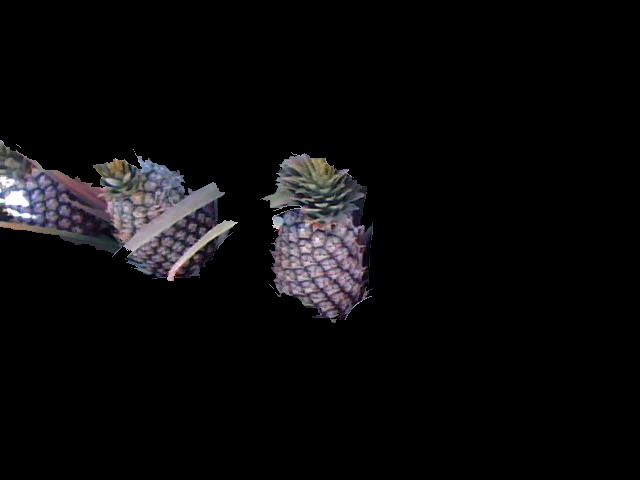
\includegraphics[width=1.4in]{figs/Waqar-DenseSeg} &
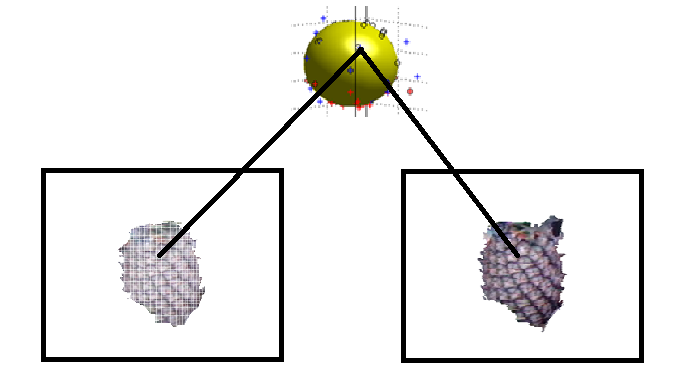
\includegraphics[width=1.5in]{figs/Waqar-Reconstruct} &
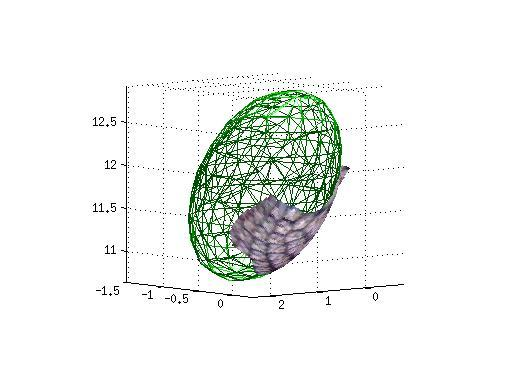
\includegraphics[width=1.4in]{figs/Waqar-Ellipsoid} \\
Dense segmentation & Optimization of spheroid & Optimized \\
with SIFT classifier & to minimize SIFT distance & spheroid
\end{tabular}

\end{frame}


\begin{frame}
\frametitle{Region-based segmentation}
\framesubtitle{Application to crop mapping}

We are working on Fast Fusion modeling of agricultural crops with
RGBD sensors:

\medskip

\begin{center}
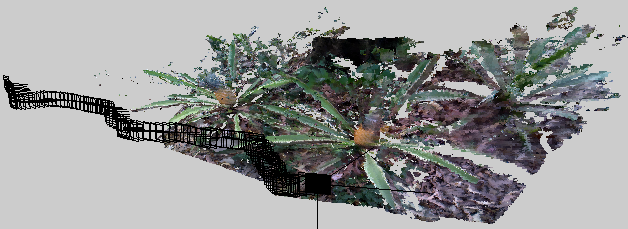
\includegraphics[width=3in]{figs/gl-world}
\end{center}

\medskip

\end{frame}


%--------------------------------------------------------------------
\section{CNNs for segmentation}
%--------------------------------------------------------------------

\begin{frame}{CNNs for segmentation}{Semantic segmentation}

  CNN models have emerged as extremely effective for region-based
  segmentation:
  \begin{itemize}
  \item \alert{Semantic segmentation} methods use fully convolutional
    networks (FCNs) to classify \alert{every pixel} in a scene.
  \item \alert{Instance segmentation} methods combine an \alert{object
    detection} pipeline with semantic segmentation inside the
    detection region.
  \end{itemize}

  \medskip
  
  Typical semantic segmentation methods:
  \begin{itemize}
  \item Object classification CNN backbone (e.g., ResNet-101) as an encoder.
    Fully connected layers are removed after training on a classification
    dataset.
  \item Optionally, the encoder's output is progressively upscaled
    with a fully convolutional decoder for spatial accuracy.
  \item Final layer gives each pixel/grid cell a meaningful object category.
  \end{itemize}

  \medskip

  Sample state of the art method: U-Net (MICCAI 2015).

\end{frame}


\begin{frame}{CNNs for segmentation}{Instance segmentation}

  \alert{Instance-aware} segmentation additionally aims to give unique
  labels to different images in the scene.

  \medskip

  One of the most effective methods is \alert{Mask R-CNN}, which
  combines Faster R-CNN with an instance mask for each region
  proposal.

  \medskip
  
  He, K., Gkioxari, G., Dollar, P., and Girshick, R. (2017), Mask
  R-CNN.  \textit{IEEE International Conference on Computer Vision
    (ICCV)}, pages 2961--2969.

  \medskip

  See also: Chen, X., Girshick, R., He, K., and Dollar, P. (2019),
  TensorMask: A Foundation for Dense Object Segmentation

\end{frame}


\begin{frame}{CNNs for segmentation}{Real time instance segmentation}

  Until recently, all deep learning instance segmentation methods were
  too slow for \alert{real time} applications.

  \medskip

  However, the first real time instance segmentation CNN,
  \alert{YOLACT}, streamlines the Mask R-CNN idea similarly to how
  YOLO streamlines Faster R-CNN.

  \medskip
  
  Bolya, D., Zhou, D., Xiao, F., and Lee, Y.J. (2019), YOLACT:
  Real-time Instance Segmentation, \textit{IEEE International
    Conference on Computer Vision (ICCV)}

\end{frame}


\begin{frame}{CNNs for segmentation}{YOLACT}

  \begin{columns}

    \column{3.2in}
    
    \myfig{3in}{bolya-fig1}{Bolya, Zhou, Xiao, and Lee (2019), Fig.\ 1}

    \column{1.8in}

    Bolya et al.\ (2019) introduce YOLACT, the fastest-ever instance
    segmentation method.

    \medskip

    29.8 mAP on the Microsoft COCO instance segmentation dataset (about
    20\% worse than Mask R-CNN).

    \medskip

    33.5 fps on a Titan Xp GPU (300\% faster than Mask R-CNN)!

  \end{columns}
  
\end{frame}


\begin{frame}{CNNs for segmentation}{YOLACT}

  Why wasn't instance segmentation real time until now?

  \medskip

  Mask R-CNN is a \alert{two-stage} method:
  \begin{itemize}
  \item Generate regions of interest (RoIs) in the first stage
  \item Classify and segment each RoI in the second stage after a
    transforming with a ROI repooling step (sequential, slow).
  \end{itemize}

  \medskip

  Bolya et al.'s idea:
  \begin{itemize}
  \item \alert{Skip localization}.
  \item Generate a dictionary of \alert{non-local prototype masks}
    over the entire image.
  \item Predict a set of \alert{linear combination coefficients} per
    instance.
  \item \alert{Linearly combine the prototypes} using predicted
    coefficients.
  \item \alert{Crop} with a predicted bounding box.
  \end{itemize}
  
\end{frame}


\begin{frame}{CNNs for segmentation}{YOLACT}

  YOLACT uses two parallel streams: FCN \alert{protonet} for
  full-image prototype masks and a \alert{prediction head} with
  per-instance prediction of mask coefficients (in addition to the
  bounding box and class predictions).
  
  \myfig{5in}{bolya-fig2}{Bolya, Zhou, Xiao, and Lee (2019), Fig.\ 2}

\end{frame}


\begin{frame}{CNNs for segmentation}{YOLACT}

  Why is this faster than Mask R-CNN?

  \medskip

  Mask R-CNN computes feature maps then region proposals.

  \medskip

  The masking part of the model has to wait for region proposal process to
  complete.

  \medskip

  By generating masks \alert{over the entire image}, masking does not
  wait for region proposals (RPs are calculated in the prediction head
  using fully connected units).

\end{frame}


\begin{frame}{CNNs for segmentation}{YOLACT}

  \medskip

  The protonet is like the output layer of a semantic segmentation FCN.

  \medskip

  The protonet's features are taken from a Feature Pyramid network then
  upsampled by a factor of $2\times 2$:

  \medskip
  
  \myfig{3in}{bolya-fig3}{Bolya, Zhou, Xiao, and Lee (2019), Fig.\ 3}

\end{frame}


\begin{frame}{CNNs for segmentation}{YOLACT}

  In addition to the two typical branches (class identity and
  bounding box parameters), the prediction head contains a third
  branch to predict $k$ mask coefficients (one for each mask in the
  protonet).

  \medskip
  
  \myfig{3in}{bolya-fig4}{Bolya, Zhou, Xiao, and Lee (2019), Fig.\ 4}

\end{frame}


\begin{frame}{CNNs for segmentation}{YOLACT}

  \begin{columns}

    \column{2.3in}
    
    \myfig{2.2in}{bolya-fig5}{Bolya, Zhou, Xiao, and Lee (2019), Fig.\ 5}

    \column{2.7in}

    Sample prototypes that emerge from training in the protonet stream.

  \end{columns}
  
\end{frame}


\begin{frame}{CNNs for segmentation}{YOLACT}

  \begin{columns}

    \column{3.8in}
    
    \myfig{3.6in}{bolya-fig6}{Bolya, Zhou, Xiao, and Lee (2019), Fig.\ 6}

    \column{1.2in}

    Several other improvements are combined: (fast non-maximum suppression
    based on parallel computation of IoU on the GPU, extra semantic segmentation
    training losses not used at runtime).

    \medskip

    Results are awesome...

  \end{columns}
    
\end{frame}


\begin{frame}{CNNs for segmentation}{YOLACT}

  Mask quality is very high:

  \medskip
  
  \myfig{5in}{bolya-fig7}{Bolya, Zhou, Xiao, and Lee (2019), Fig.\ 7}

\end{frame}


\begin{frame}{CNNs for segmentation}{YOLACT}

  More results:

  \medskip
  
  \myfig{3.3in}{bolya-fig8}{Bolya, Zhou, Xiao, and Lee (2019), Fig.\ 8}

\end{frame}


\end{document}

